% Grundkurs Digitaltechnik - das gedruckte Handbuch.
%
%   make          -> grundkurs.pdf
%
% Die Kapitel unter kapitel/ sind der einmalige Auszug aus dem Word-Manuskript
% von 2004 (tools/convert-book.js). Ab jetzt werden sie hier gepflegt; die
% Webfassung unter book/ ist eine eigenstaendige zweite Fassung und wird
% NICHT aus dieser hier erzeugt.

\documentclass[
  11pt,
  ngerman,
  numbers=noenddot,
  listof=totoc,
  bibliography=totoc,
  twoside,
  open=right,
]{scrbook}

% Satzspiegel, Schrift und Pakete des gedruckten Handbuchs.
%
% Diese Datei ist handgepflegt. Der Buchkoerper unter kapitel/ stammt aus dem
% einmaligen Lauf von tools/convert-book.js, die Gestaltung hier nicht.

\usepackage{fontspec}
\usepackage[ngerman]{babel}
\usepackage{csquotes}
\usepackage{microtype}

% Libertinus statt Inter. Der Plan sah Inter vor, damit Buch und Website
% dasselbe Schriftbild bekommen - im Repo liegt Inter aber nur als woff2
% (common/public/css/inter/), und das kann fontspec nicht einbinden. Eine
% Serifenschrift traegt einen 100-Seiten-Fliesstext im Druck ohnehin besser als
% eine Oberflaechen-Grotesk. Falls Inter doch gewuenscht ist: woff2 mit fonttools
% nach otf wandeln, dann hier eintragen.
\setmainfont{Libertinus Serif}
\setsansfont{Libertinus Sans}
\setmonofont{Libertinus Mono}

\usepackage{amsmath}
\usepackage{graphicx}
\graphicspath{{media/}}

% Logiktafeln. booktabs setzt Linien mit Abstand statt Gitter - bei
% Wahrheitstabellen aus Nullen und Einsen ist das der Unterschied zwischen
% lesbar und Tapete.
\usepackage{booktabs}
\renewcommand{\arraystretch}{1.15}

\usepackage[
  a5paper,
  inner=20mm, outer=15mm, top=18mm, bottom=20mm,
]{geometry}

% 56 Stichwoerter, aus den XE-Feldern des Manuskripts uebernommen.
\usepackage{imakeidx}
\makeindex[title=Stichwortverzeichnis, intoc]

\usepackage[hidelinks]{hyperref}

% Abbildungen sitzen mitten im Text und sollen dort bleiben.
\setkomafont{caption}{\small}
\setkomafont{captionlabel}{\small\bfseries}
\setcapindent{0pt}


\title{Grundkurs Digitaltechnik}
% Untertitel war im Manuskript "Grundlagen fuer den DigitalSimulator" - das
% Programm, fuer das das Buch 1:1 als Handbuch geschrieben wurde.
\subtitle{Grundlagen für Electra.Academy}
\author{Andreas Herz}
\date{\the\year}

\begin{document}

\frontmatter
\maketitle
\tableofcontents

\mainmatter

\chapter{Grundlagen}

In der Schwachstromelektronik werden heute die beiden Bereiche Analog-Technik und Digital-Technik unterschieden.\index{Schwachstromelektronik}

Ein einfaches Beispiel für diese beiden Begriffe stellt ein gewöhnlicher Spannungsmesser dar. Wenn man das Messgerät wie in Abb. 1 an eine regelbare Spannungsquelle anschließt, so vergrößert sich der Zeigerausschlag mit zunehmender Spannung. Dabei wird einem bestimmten Spannungswert genau eine Zeigerstellung zugeordnet. Dieser gleichmäßige Anstieg oder Abfall des Zeigers wird analoges Verhalten genannt.\index{Spannungsmesser}\index{Spannungsquelle}\index{Spannung}\index{Spannungswert}

\begin{figure}[htbp]
  \centering
  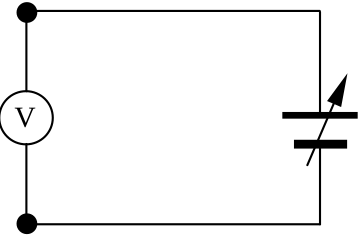
\includegraphics[width=.8\linewidth]{media/abb-02}
  \caption{Spannungsmesser}
\end{figure}

Dabei ist jeder Zwischenwert der Spannung innerhalb des Messbereiches des Spannungsgerätes möglich. Der Ausschlag des Messgerätes entspricht dabei der angelegten Spannung, oder anders ausgedrückt: die angelegte Spannung ist analog zum Zeigerausschlag.\index{Spannung}\index{Spannungsgerätes}

Abb. 2 zeigt ein typisches Diagramm für analoges Verhalten. Hier ist der Zeigerausschlag des Messgerätes in Abhängigkeit der Zeit t dargestellt. Es ist deutlich zu sehen, dass jeder beliebige Zwischenwert des Ausschlags eingestellt werden kann.

\begin{figure}[htbp]
  \centering
  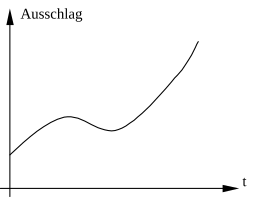
\includegraphics[width=.8\linewidth]{media/abb-03}
  \caption{Analog Diagramm}
\end{figure}

Bei der Digital-Technik dagegen wird die Information, die bei der Analog-Technik durch den Kurvenverlauf gegeben ist (Zeigerausschlag), durch das Ablesen auf der Skala bestimmt. Man ordnet eben jedem Zeigerstand einen bestimmten Spannungswert zu. Das ist bei fast allen Messgeräten durch die Skala von vornherein schon gegeben. Indem man nun die Skalenstriche abzählt, setzt man das analoge Signal (Ausschlag des Zeigers) in ein digitales Signal (Anzahl der Striche) um. \index{Kurvenverlauf}\index{Spannungswert}\index{analoge Signal}\index{digitales Signal}

Dabei hat die Digital-Technik gegenüber der Analog-Technik einen großen Vorteil. Während bei analogen Schaltungen der Spannungsbereich meist genau stimmen muss, braucht man in digitalen Schaltungen nur den richtigen Spannungsbereich einzuhalten. Dies bringt eine erhöhte Stabilität der digitalen Schaltungen mit sich.

Die beiden Spannungsbereiche, die in der Digital-Technik verwendet werden, heißen L-Bereich (von engl.: low = niedrig) und H-Bereich (von engl.: high = hoch). Hier werden für die Beispiele eine Versorgungsspannung U\textsubscript{v} = 5V und die beiden Spannungsbereiche mit 0V bis +0,5V für L (low) und +2,5V bis +5V für H (high) festgelegt, da diese Spannungsbereiche außerdem gerade für TTL-Schaltungen (TTL = Transistor-Transistor-Logik) oft benötigt werden.\index{Spannungsbereiche}\index{H-Bereich}

In der mathematischen Beschreibung von digitalen Schaltungen wird der L-Bereich mit 0 und der H-Bereich mit 1 beschrieben. Dies ist unter anderem für Wahrheitstabellen und KV-Tafeln, die in anderen Kapiteln zur Anwendung kommen, sehr von Vorteil.\index{H-Bereich}\index{Wahrheitstabellen}\index{KV-Tafeln}


\chapter{Das Dualsystem}

In den digitalen Schaltungen mit seinen zwei Bereichen H und L wird das Dualsystem für die Beschreibung mathematischer Zusammenhänge angewendet. Dabei werden nur zwei Zahlen benötigt, nämlich 1 und 0. Eine Verdeutlichung des Dualsystems ist am einfachsten durch eine Gegenüberstellung mit unserem üblichen Dezimalsystem zu erreichen:\index{Dualsystem}\index{Dualsystems}\index{Dezimalsystem}

\begin{table}[htbp]
  \centering
  \begin{tabular}{cc}
    \toprule
    \textbf{Dezimalsystem} & \textbf{Dualsystem} \\
    \midrule
     0 &  0 \\
     1 &  1 \\
     2 &  10 \\
     3 &  11 \\
     4 &  100 \\
     5 &  101 \\
     6 &  110 \\
     7 &  111 \\
     8 &  1000 \\
     9 &  1001 \\
     10 &  1010 \\
     11 &  1011 \\
    \bottomrule
  \end{tabular}
  \par\medskip usw.
\end{table}

Dabei spricht man die duale Zahl 1001 nicht etwa „Eintausendeins“, sondern man spricht die Zahlen einzeln von links beginnend, also „Eins, Null, Null, Eins“.

Durch diese Darstellung können digitale Schaltungen (z.B. Zähler) sehr einfach und durchsichtig dargestellt werden.


\chapter{Vorbemerkungen}

Alle hier behandelten Schaltungen entsprechen der sog. Positiv-Logik. Das heißt, dass der H-Bereich eine positive Spannung sein muss. Es gibt auch eine Negativ-Logik, die aber in der Technik kaum eine Bedeutung hat.\index{Positiv-Logik}\index{H-Bereich}\index{Spannung}\index{Negativ-Logik}

Weiterhin gilt ein „offener“ Eingang (nicht angeschlossener Eingang) immer als Wert 1 (entspr. H). Dies ist durch die Bauweise der ICs (Integrierte Schaltungen) bedingt, die intern immer den Wert 1 an einen Ausgang legen, wenn dieser nicht angeschlossen ist. Das bringt vor allem beim Zusammenschalten mehrerer Verknüpfungsschaltungen enorme Vorteile.\index{Integrierte Schaltungen}\index{Verknüpfungsschaltungen}

Der Masseanschluss bei digitalen Schaltungen hat immer den Wert 0. Dies entspricht bei der Stromversorgung dem Minuspol. Der Wert 1 ist also der Pluspol der Spannungsquelle. Falls Messungen mit einem Spannungsmessgerät oder gar Oszilloskop gemacht werden, ist daher der Massepunkt immer der negative Pol der Spannungsquelle. Die kapazitive Last für digitale Schaltungen sollte 100 pF nicht überschreiten, damit die Funktion gewährleistet ist und eine Überlast der Ausgänge durch zu hohe Auf- bzw. Entladeströme vermieden wird. Sind größere Kondensatoren zur Signalverzögerung erforderlich, so ist ein Vorwiderstand vorzusehen.\index{Masseanschluss}\index{Spannungsquelle}\index{Spannungsmessgerät}\index{Oszilloskop}\index{kapazitive Last}\index{Signalverzögerung}

Der Ausgangsstrom von TTL-Schaltungen ist sehr gering, meist bei 20 mA. Das reicht wohl für den Betrieb einer Kontroll-LED (Licht Emittierende Diode = Leuchtdiode), doch ist darauf zu achten, dass der Ausgang nicht überlastet wird. Notfalls muss ein Schaltverstärker dem Ausgang folgen, der das Ausgangssignal verstärkt. Bei manchen IC’s jedoch ist speziell für LED-Betrieb ein Treiber vorhanden, der einen Anschluss von mehr als einer LED erlaubt (z.B. beim 7-Segment-Decoder). Es ist ratsam, sich deshalb in einem Datenbuch über diesen Sachverhalt zu informieren.\index{Ausgangsstrom}\index{LED}\index{Ausgangssignal}\index{Treiber}


\chapter{Verknüpfungsschaltungen}

\section{Einführung}

Logische Verknüpfungsschaltungen sind das Grundgerüst der digitalen Technik. Mit Hilfe der 5 hier aufgeführten Verknüpfungsschaltungen, die auch Gatter genannt werden, lassen sich nun alle anderen Verknüpfungsschaltungen realisieren.\index{Verknüpfungsschaltungen}\index{Gatter}

Die Wahrheitstabelle, oder auch Logik-Tafel, die bei jeder Verknüpfungsschaltung mit aufgeführt wird, gibt an, welches Signal am Ausgang anliegt, nachdem die Eingänge in einer bestimmten Weise angeschlossen wurden. Dabei werden alle möglichen Anschlusskombinationen durchgespielt.\index{Wahrheitstabelle}

\section{AND-Gatter (UND-Verknüpfung)}

Die Boolesche Funktionsgleichung (mathematische Gleichung) für das AND-Gatter lautet:\index{AND}\index{Gatter}

\begin{quote}
  A = E\textsubscript{1} \ensuremath{\wedge} E\textsubscript{2}  (sprich: „E\textsubscript{1} und E\textsubscript{2}“)
\end{quote}


Das bedeutet, dass A nur dann den Wert 1 hat, wenn die Eingänge E\textsubscript{1} und E\textsubscript{2} den Wert 1 haben. In allen anderen Fällen hat der Ausgang A den Wert 0. Anhand der Logik-Tafel ist dies leicht zu erkennen. In der Zeile, in der A den Wert 1 hat, haben die beiden Eingänge ebenfalls den Wert 1.

\begin{table}[htbp]
  \centering
  \caption{Logiktafel AND-Gatter}
  \begin{tabular}{ccc}
    \toprule
    E\textsubscript{1} & E\textsubscript{2} & A \\
    \midrule
    0 & 0 & 0 \\
    0 & 1 & 0 \\
    1 & 0 & 0 \\
    1 & 1 & 1 \\
    \bottomrule
  \end{tabular}
\end{table}

\begin{figure}[htbp]
  \centering
  
\includegraphics[width=.8\linewidth]{media/abb-04}
  \caption{Schaltsymbol AND}
\end{figure}

Hier ist die einfachste UND-Verknüpfung gewählt worden, nämlich die mit 2 Eingängen. Tatsächlich gibt es jedoch auch AND-Gatter mit mehr  als zwei Eingängen. Die mathematische Logik bleibt dabei aber gleich: Nur wenn alle Eingänge den Wert 1 haben, hat der Ausgang ebenfalls den Wert 1.\index{AND}\index{Gatter}

Die UND-Verknüpfung wird auch als „Konjunktion“ bezeichnet, was so viel heißt wie „Bindung“.\index{Konjunktion}

\section{OR-Gatter (ODER-Verknüpfung)}

Hier heißt die mathematischer Gleichung:

\begin{quote}
  A = E1 \ensuremath{\vee} E2  (sprich: „E1 oder E2“)
\end{quote}


Dabei hat A dann den Wert 1, wenn E\textsubscript{1} oder E\textsubscript{2} oder beide (!) Eingänge den Wert 1 haben. Dieses Verhalten unterscheidet sich von dem normalen Sprachgebrauch des Wortes „oder“. Hier bedeutet es: A hat nur dann den Wert 0, wenn beide Eingänge den Wert 0 haben. Sonst hat der Ausgang den Wert 1.

\begin{table}[htbp]
  \centering
  \caption{Logiktafle OR-Gatter}
  \begin{tabular}{ccc}
    \toprule
    E\textsubscript{1} & E\textsubscript{2} & A \\
    \midrule
    0 & 0 & 0 \\
    0 & 1 & 1 \\
    1 & 0 & 1 \\
    1 & 1 & 1 \\
    \bottomrule
  \end{tabular}
\end{table}

\begin{figure}[htbp]
  \centering
  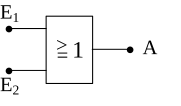
\includegraphics[width=.8\linewidth]{media/abb-05}
  \caption{Schaltsymbol OR}
\end{figure}

Die ODER-Verknüpfung gibt es ebenfalls mit mehr als zwei Eingängen, wobei sich die mathematischer Logik wie beim AND-Gatter nicht ändert. Eine andere Bezeichnung für das OR-Gatter ist die „Disjunktion“, das heißt „Trennung“.\index{ODER-Verknüpfung}\index{AND}\index{Gatter}\index{OR-Gatter}\index{Disjunktion}

\section{INVERTER (NOT-Verknüpfung)}

Das Schaltsymbol des Inverters ist unten abgebildet. Dabei lässt sich die mathematische Logik durch folgende Gleichung darstellen:\index{Inverters}

\begin{quote}
  A = \ensuremath{\lnot}E (sprich „E komplementär“ oder „E negiert“).
\end{quote}
\index{komplementär}

\begin{table}[htbp]
  \centering
  \caption{Logiktafel NOT-Gatter}
  \begin{tabular}{cc}
    \toprule
    E & A \\
    \midrule
    0 & 1 \\
    1 & 0 \\
    \bottomrule
  \end{tabular}
\end{table}

\begin{figure}[htbp]
  \centering
  
\includegraphics[width=.8\linewidth]{media/abb-06}
  \caption{Schaltsymbol NOT}
\end{figure}

Ein anderer Begriff für den Inverter ist die „Negation“. Indem man nun das AND-Gatter und das OR-Gatter negiert, erhält man zwei weitere wichtige Verknüpfungsschaltungen.\index{Negation}\index{AND}\index{Gatter}\index{OR-Gatter}\index{Verknüpfungsschaltungen}

\section{NAND-Gatter}

Gebildet aus den englischen Worten „not and“, also „nicht und“. Daraus lässt sich bereits schließen, dass die Verknüpfung negiert sein muss. Die mathematische Gleichung bestätigt dies:

\begin{quote}
  A = \ensuremath{\lnot}(E\textsubscript{1} \ensuremath{\wedge} E\textsubscript{2}) (sprich: „E\textsubscript{1} und E\textsubscript{2} negiert“)
\end{quote}


Der Ausgang A hat immer den Wert 1, außer wenn beide Eingänge den Wert 1 haben. Anhand der Logik-Tafel lässt sich auch erkennen, dass die NAND-Funktion an ihrem Ausgang genau das entgegengesetzte Signal hat wie das AND-Gatter.\index{AND}\index{Gatter}

\begin{table}[htbp]
  \centering
  \caption{Logiktafel NAND-Gatter}
  \begin{tabular}{ccc}
    \toprule
    E\textsubscript{1} & E\textsubscript{2} & A \\
    \midrule
    0 & 0 & 1 \\
    0 & 1 & 1 \\
    1 & 0 & 1 \\
    1 & 1 & 0 \\
    \bottomrule
  \end{tabular}
\end{table}

\begin{figure}[htbp]
  \centering
  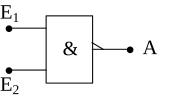
\includegraphics[width=.8\linewidth]{media/abb-07}
  \caption{Schaltsymbol NAND}
\end{figure}

\section{NOR-Gatter}

Gebildet aus den englischen Wörtern „not or“, was übersetzt „nicht oder“ heißt. Es handelt sich also wiederum um eine Negation, nämlich die der OR-Verknüpfung. Die mathematische Gleichung lautet:\index{Negation}

A = \ensuremath{\lnot}(E\textsubscript{1} \ensuremath{\vee} E\textsubscript{2}) (sprich: „E\textsubscript{1} oder E\textsubscript{2} negiert“)

Bei dieser Verknüpfungsschaltung hat der Ausgang A den Wert 1, wenn beide Eingänge den Wert 0 haben. In allen anderen Fällen hat der Ausgang den Wert 0.

\begin{table}[htbp]
  \centering
  \caption{Logiktafle NOR-Gatter}
  \begin{tabular}{ccc}
    \toprule
    E\textsubscript{1} & E\textsubscript{2} & A \\
    \midrule
    0 & 0 & 1 \\
    0 & 1 & 0 \\
    1 & 0 & 0 \\
    1 & 1 & 0 \\
    \bottomrule
  \end{tabular}
\end{table}

\begin{figure}[htbp]
  \centering
  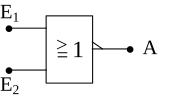
\includegraphics[width=.8\linewidth]{media/abb-08}
  \caption{Schaltsymbol NOR}
\end{figure}

Da diese beiden letzten Gatter sehr häufig vorkommen, haben sie ein eigenes Schaltsymbol. Außerdem sind sie für den Praktiker sehr interessant, da sie gegenüber den UND- bzw. ODER-Gattern meist erheblich billiger sind. Deshalb nimmt man häufig zwei NAND-Gatter um ein UND-Gatter billig aufzubauen, oder zwei NOR-Gatter für ein OR-Gatter. Die dafür notwendigen Schaltungen werden im Folgenden erklärt.\index{NAND-Gatter}\index{OR-Gatter}

\begin{figure}[htbp]
  \centering
  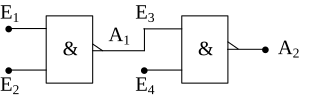
\includegraphics[width=.8\linewidth]{media/abb-09}
  \caption{Schaltbild UND-Gatter aus zwei NAND-Gatter}
\end{figure}

Bei dieser Schaltung hat der Ausgang A\textsubscript{1} nur dann den Wert 0, wenn beide Eingänge, also E\textsubscript{1} und E\textsubscript{2 }den Wert 1 haben. Der offene (nicht angeschlossene) Eingang E\textsubscript{4} hat generell den Wert 1. Um aber am Ausgang A\textsubscript{2} den Wert 1 zu erreichen, muss deswegen E\textsubscript{3} und somit am Ausgang A\textsubscript{1} der Wert 0 anliegen. Dies wird, wie oben schon beschrieben, nur dadurch erreicht, dass man den Eingängen E\textsubscript{1} und E\textsubscript{2} den Wert 1 zuordnet.

Mathematisch ausgedrückt bedeutet dies:

\begin{quote}
  A\textsubscript{1} = \ensuremath{\lnot}(E\textsubscript{1 }\ensuremath{\wedge} E\textsubscript{2})
\end{quote}


\begin{quote}
  A\textsubscript{2} = \ensuremath{\lnot}A\textsubscript{1} = \ensuremath{\lnot}(\ensuremath{\lnot}(E\textsubscript{1 }\ensuremath{\wedge} E\textsubscript{2}))
\end{quote}


\ensuremath{\lnot}(\ensuremath{\lnot}(E\textsubscript{1 }\ensuremath{\wedge} E\textsubscript{2})) ist aber nichts anderes als E\textsubscript{1 }\ensuremath{\wedge} E\textsubscript{2}; somit gilt die Funktionsgleichung der normalen UND-Verknüpfung:

\begin{quote}
  A\textsubscript{2} = E\textsubscript{1 }\ensuremath{\wedge} E\textsubscript{2}
\end{quote}


Dies beweist, dass die obige Schaltung einer normalen UND-Verknüpfung entspricht.

\begin{figure}[htbp]
  \centering
  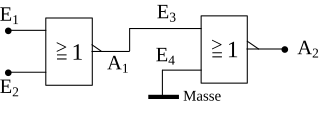
\includegraphics[width=.8\linewidth]{media/abb-10}
  \caption{Schaltbild OR-Gatter aus zwei NOR-Gatter}
\end{figure}

Die Logik dieser Schaltung ist ähnlich der Vorherigen. Der Ausgang A\textsubscript{2} hat nur dann den Wert 0, wenn E\textsubscript{3} den Wert 1 hat. E\textsubscript{4} ist durch den Masseanschluss sowieso immer auf 0. Der Wert 1 an E\textsubscript{3} und somit an A\textsubscript{1} wird aber nur erreicht, indem man E\textsubscript{1} und E\textsubscript{2} den Wert 0 zuordnet. In allen anderen Fällen hat A\textsubscript{1} den Wert 0 und damit A\textsubscript{2} den Wert 1. Dies wiederum entspricht genau der OR-Verknüpfung.\index{Masseanschluss}

Hier der mathematische Beweis:

\begin{quote}
  A\textsubscript{1} = \ensuremath{\lnot}(E\textsubscript{1 }\ensuremath{\vee} E\textsubscript{2})
\end{quote}


\begin{quote}
  A\textsubscript{2} = \ensuremath{\lnot}A\textsubscript{1} = \ensuremath{\lnot}(\ensuremath{\lnot}(E\textsubscript{1 }\ensuremath{\vee} E\textsubscript{2})) = E\textsubscript{1 }\ensuremath{\vee} E\textsubscript{2}
\end{quote}


Mit diesen nun beschriebenen 5 Grundschaltungen (AND-, NAND-, OR-, NOR-Gatter und Inverter) lassen sich alle anderen logischen Verknüpfungsschaltungen realisieren. Man muss nur die gewünschten Elemente zusammenschalten. Den mathematischen Hintergrund für die Kombination der Gatter liefert die Boolesche Algebra. Die Grundfunktionen sind bei der Erklärung der Schaltungen mit angegeben.\index{Grundschaltungen}\index{Verknüpfungsschaltungen}

\section{EX-OR-Gatter (Exklusiv-ODER)}

Eine Variation der Zusammenschaltung der 5 Grundgatter ist das Exklusiv-ODER. Im Gegensatz zur ODER-Verknüpfung tritt am Ausgang nicht der Wert 1 auf, wenn beide Eingänge den Wert 1 haben. Diese Funktion entspricht jetzt dem „oder“ wie es im normalen Sprachgebrauch verwendet wird. Das heißt, dass am Ausgang der Wert 1 vorliegt, wenn E\textsubscript{1} oder E\textsubscript{2} den Wert 1 haben. Sobald E\textsubscript{1} und E\textsubscript{2} den gleichen Wert haben, liegt am Ausgang A der Wert 0.\index{Exklusiv-ODER}\index{ODER-Verknüpfung}

\begin{table}[htbp]
  \centering
  \caption{Logiktafel Ex-OR-Gatter}
  \begin{tabular}{ccc}
    \toprule
    E\textsubscript{1} & E\textsubscript{2} & A \\
    \midrule
    0 & 0 & 0 \\
    0 & 1 & 1 \\
    1 & 0 & 1 \\
    1 & 1 & 0 \\
    \bottomrule
  \end{tabular}
\end{table}

\begin{figure}[htbp]
  \centering
  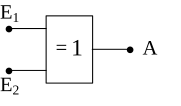
\includegraphics[width=.8\linewidth]{media/abb-11}
  \caption{Schaltsymbol EX-OR-Gatter}
\end{figure}

Da diese Verknüpfungsschaltung sehr häufig vorkommt, hat auch sie ihr eigenes Schaltsymbol. Sie kann aber auch durch die Zusammenschaltung von 2 Invertern, 2 AND-Gattern und einem NOR-Gatter aufgebaut werden. Die mathematische Funktion lautet:

\begin{quote}
  A = (\ensuremath{\lnot}E\textsubscript{1} \ensuremath{\wedge} E\textsubscript{2}) \ensuremath{\vee} (E\textsubscript{1} \ensuremath{\wedge} \ensuremath{\lnot}E\textsubscript{2})
\end{quote}


Nun zum Schaltbild des Exklusiv-ODER. Ein Praktiker kann schon anhand der mathematischen Gleichung das Schaltbild zeichnen. Man muss dabei nur genau die Gleichung in die Schaltsymbole der logischen Verknüpfung umwandeln.\index{Exklusiv-ODER}

\begin{figure}[htbp]
  \centering
  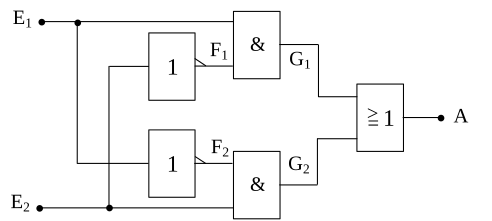
\includegraphics[width=.8\linewidth]{media/abb-12}
  \caption{Schaltbild EX-OR-Gatter}
\end{figure}

Bei dieser Schaltung wollen wir nun einmal einen anderen Weg gehen, der sich vor allem bei komplexen und komplizierteren Schaltungen als sehr einfach herausstellt. Dabei wird an die beiden Eingänge E\textsubscript{1} und E\textsubscript{2} jede mögliche Eingangskombination gelegt und bis zum Ausgang A „durchgespielt“. Im vorliegenden Fall sind das genau 4 Kombinationen.

An E\textsubscript{1} und E\textsubscript{2} liegt jeweils der Wert 0. Das obere AND-Gatter hat also am Eingang den Wert 0 von E\textsubscript{1} und den Wert 1 vom invertierten E\textsubscript{2}. Das ergibt einen Zwischenwert G\textsubscript{1} = 0. Das untere AND-Gatter hat ebenfalls den Wert 0 (von E\textsubscript{2}) und den Wert 1 (invertiertes E\textsubscript{1}) und somit ebenfalls den Zwischenwert G\textsubscript{2} = 0. Diese beiden Zwischenwerte liegen nun an einem OR-GATTER, das dadurch am Ausgang den Wert 0 hat. Damit ist die erste Zeile der Logik-Tafel schon festgelegt.\index{AND}\index{AND-Gatter}

Nun legt man an E\textsubscript{1} den Wert 0 und an E\textsubscript{2} den Wert 1. Da E\textsubscript{2} invertiert an das obere AND-Gatter gelangt und E\textsubscript{1} von vorneherein 0 ist, erscheint am oberen Zwischenausgang G\textsubscript{1} der Wert 0. Beim unteren AND-Gatter sind dagegen beide Eingänge auf dem Wert 1, da E\textsubscript{1} invertiert wird und E\textsubscript{2} den Wert 1 hat. Das ergibt am Zwischenausgang G\textsubscript{2} den Wert 1. Am OR-Gatter liegt also nun einmal der Wert 0 (G\textsubscript{1}) und einmal der Wert 1 (G\textsubscript{2}). Der Ausgang A hat somit den Wert 1.\index{AND}\index{AND-Gatter}\index{OR-Gatter}

Wenn man nun an den Eingang E\textsubscript{1} den Wert 1 und an E\textsubscript{2} den Wert 0 legt, so läuft die Logik genau den gleichen Weg. Nur liegen dabei die Werte die vorher am oberen AND-Gatter lagen nun am unteren und umgekehrt. Am Ausgang erscheint deshalb wie unter 2. der Wert 1.\index{AND}

Die letzte Kombinationsmöglichkeit ist nun die, dass beide Eingänge E\textsubscript{1} und E\textsubscript{2} den Wert 1 bekommen. Durch die Invertierung von E\textsubscript{2} am oberen und E\textsubscript{1} am unteren AND-Gatter haben die Zwischenausgänge G\textsubscript{1} und G\textsubscript{2} die gleichen Werte, nämlich 0. Eine Parallele dazu ist die erste Kombination. Am Ausgang A erscheint deshalb der Wert 0.\index{AND}

\section{EX-NOR-Gatter}

Eine Variation des EX-OR-Gatters ist diese Schaltung. Dabei wird nur der Ausgang A der oberen Schaltung invertiert.

\begin{table}[htbp]
  \centering
  \caption{Logiktafel EX-NOR-Gatter}
  \begin{tabular}{ccc}
    \toprule
    E\textsubscript{1} & E\textsubscript{2} & A \\
    \midrule
    0 & 0 & 1 \\
    0 & 1 & 0 \\
    1 & 0 & 0 \\
    1 & 1 & 1 \\
    \bottomrule
  \end{tabular}
\end{table}

\begin{figure}[htbp]
  \centering
  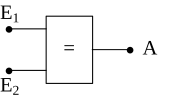
\includegraphics[width=.8\linewidth]{media/abb-13}
  \caption{Schaltsymbol EX-NOR-Gatter}
\end{figure}

\begin{figure}[htbp]
  \centering
  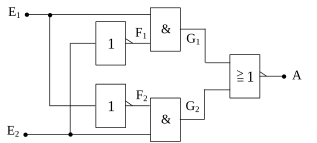
\includegraphics[width=.8\linewidth]{media/abb-14}
  \caption{Schaltbild EX-NOR-Gatter}
\end{figure}

\section{Gatter mit mehreren Eingängen}

Oftmals ist es nötig, Verknüpfungsschaltungen mit 3 oder 4 Eingängen in eine Schaltung zu integrieren. Haben Sie diese Gatter nicht zur Hand, so kann man sie mit den unten abgebildeten Schaltungen aufbauen.\index{Verknüpfungsschaltungen}\index{Gatter}

Zuerst die AND-Verknüpfung mit 3 Eingängen. Die folgende Tabelle zeigt, dass die abgebildete Schaltung einem AND-Gatter mit 3 Eingängen entspricht. Eingezeichnet sind auch die Zwischenausgänge Z\textsubscript{1}, Z\textsubscript{2} und Z\textsubscript{3}.

\begin{table}[htbp]
  \centering
  \begin{tabular}{ccccccc}
    \toprule
    E\textsubscript{1} & E\textsubscript{2} & E\textsubscript{3} & Z\textsubscript{1} & Z\textsubscript{2} & Z\textsubscript{3} & A \\
    \midrule
    0 & 0 & 0 & 1 & 0 & 1 & 0 \\
    0 & 0 & 1 & 1 & 0 & 1 & 0 \\
    0 & 1 & 0 & 1 & 0 & 1 & 0 \\
    0 & 1 & 1 & 1 & 0 & 1 & 0 \\
    1 & 0 & 0 & 1 & 0 & 1 & 0 \\
    1 & 0 & 1 & 1 & 0 & 1 & 0 \\
    1 & 1 & 0 & 0 & 1 & 1 & 0 \\
    1 & 1 & 1 & 0 & 1 & 0 & 1 \\
    \bottomrule
  \end{tabular}
\end{table}

\begin{figure}[htbp]
  \centering
  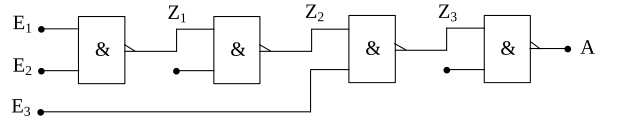
\includegraphics[width=.8\linewidth]{media/abb-15}
  \caption{Schaltbild AND-Gatter mit 3 Eingänge aus NAND-Gattern}
\end{figure}

Nach diesem Schema lässt sich auch eine UND-Schaltung mit 4 Eingängen aus 6 NAND-Gattern aufbauen usw.

NOR-Gatter mir 3 Eingängen aus 3 NOR-Gattern

Die folgende Logiktafel mit den Zwischenausgängen gibt auch hier wiederum Auskunft darüber, dass das Verhalten der Schaltung dem eines NOR-Gatters mit 3 Eingängen entspricht.

\begin{table}[htbp]
  \centering
  \begin{tabular}{cccccc}
    \toprule
    E\textsubscript{1} & E\textsubscript{2} & E\textsubscript{3} & Z\textsubscript{1} & Z\textsubscript{2} & A \\
    \midrule
    0 & 0 & 0 & 1 & 0 & 1 \\
    0 & 0 & 1 & 1 & 0 & 0 \\
    0 & 1 & 0 & 0 & 1 & 0 \\
    0 & 1 & 1 & 0 & 1 & 0 \\
    1 & 0 & 0 & 0 & 1 & 0 \\
    1 & 0 & 1 & 0 & 1 & 0 \\
    1 & 1 & 0 & 0 & 1 & 0 \\
    1 & 1 & 1 & 0 & 1 & 0 \\
    \bottomrule
  \end{tabular}
\end{table}

\begin{figure}[htbp]
  \centering
  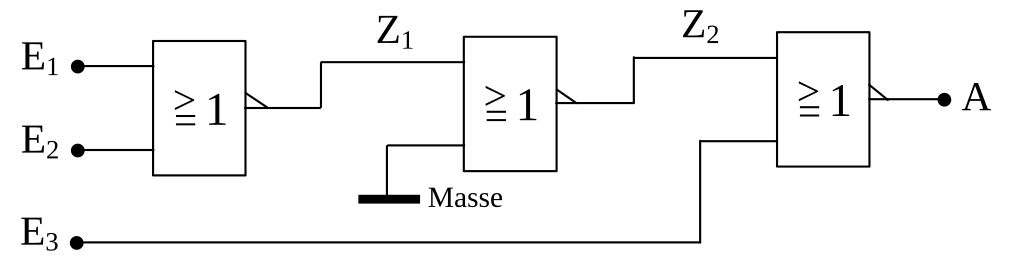
\includegraphics[width=.8\linewidth]{media/abb-16}
  \caption{Schaltbild NOR-Gatter mit 3 Eingängen aus 3 NOR-Gatter}
\end{figure}

Auch bei dieser Schaltung lassen sich durch Hinzufügen weiterer NOR-Gatter Schaltungen erzeugen, die sich wie große NOR-Gatter mit noch mehr Eingängen verhalten.

\section{Kombi-Schaltungen}

Neben den bisher gezeigten Verknüpfungsschaltungen gibt es noch weitere Schaltsymbole für spezielle Kombinationen. Daher der Name Kombi-Schaltungen. Sie werden in dieser Form sehr häufig für Decoder und andere logische Schaltungen benötigt. Aus diesem Grunde hat man auch für sie vereinfachte Darstellungen gefunden.\index{Verknüpfungsschaltungen}

1. Zwei OR-Gatter, deren Ausgänge über ein AND-Gatter verknüpft sind:\index{AND-Gatter}

\begin{figure}[htbp]
  \centering
  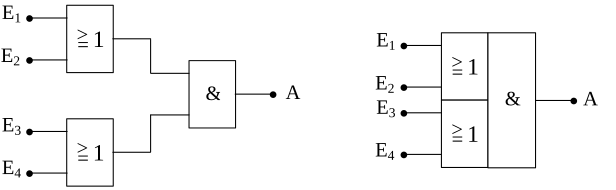
\includegraphics[width=.8\linewidth]{media/abb-17}
  \caption{Schaltbild Kombischaltung OR/AND}
\end{figure}

\textbf{2. AND}\textbf{-Gatter, das mit einem OR-Gatter}\textbf{ verknüpft ist:}\index{AND}\index{OR-Gatter}

\begin{figure}[htbp]
  \centering
  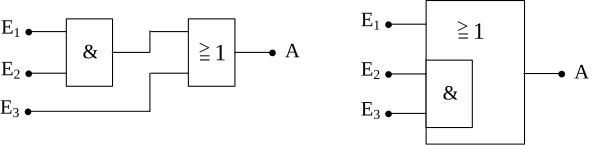
\includegraphics[width=.8\linewidth]{media/abb-18}
  \caption{Schaltbild Kombischaltung AND/OR}
\end{figure}

\textbf{3. AND-Gatter verknüpft mit einem OR-Gatter}\textbf{ (3 Eingänge) und nachgeschaltetem AND-Gatter}\index{OR-Gatter}\index{AND-Gatter}

\begin{figure}[htbp]
  \centering
  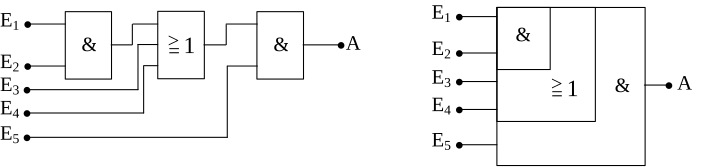
\includegraphics[width=.8\linewidth]{media/abb-19}
  \caption{Schaltbild Kombischaltung AND/NOR/AND}
\end{figure}

4. Zwei AND-Gatter, deren Ausgänge durch ein OR-Gatter miteinander verknüpft sind:\index{OR-Gatter}

\begin{figure}[htbp]
  \centering
  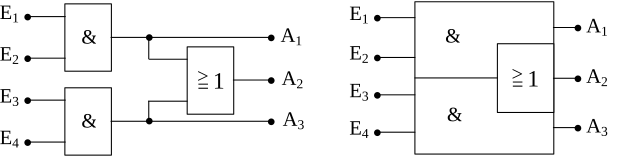
\includegraphics[width=.8\linewidth]{media/abb-20}
  \caption{Schaltbild Kombischaltung AND/NOR}
\end{figure}


\chapter{Taktgeber}

\section{Einführung}

Der Taktgeber ist besonders für die im folgenden beschriebenen Flipflops, Zähler und Speicher von Nutzen. Dazu wird jeder Zeitabschnitt im Programmablauf einer digitalen Schaltung in Taktimpulse eingeteilt. Der Takt wird durch einen dauernden Wechsel von H und L, dem sogenannten Dauerimpuls, an eine Schaltung gelegt. So z.B. auch an jedem Computer. Für Versuchsschaltungen und zur genauen Verfolgung der Schaltzustände ist es von Vorteil, wenn die Taktlänge variabel ist. Man kann dadurch langsam den Programmablauf der Schaltung kontrollieren oder schnell das Verhalten prüfen.\index{Taktgeber}

Eine solche Schaltung für schnelle Taktimpulse ist in Abb. 20 dargestellt. Es ist ein astabiler Multivibrator mit 2 Kondensatoren die zwischen 22 nF und 1 µF liegen und mit 2 Widerständen die zweckmässigerweise wegen der Impulslänge als Drehpotentiometer verwendet werden. Man wählt am besten Drehpotentiometer in der Grössenordnung von 3,3 k. Weiterhin werden 2 Inverter verwendet.\index{Multivibrator}

\begin{figure}[htbp]
  \centering
  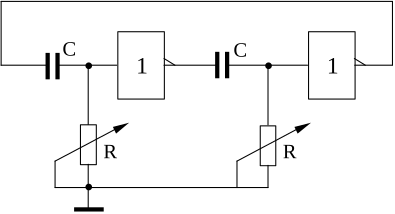
\includegraphics[width=.8\linewidth]{media/abb-21}
  \caption{Schaltbild Taktgeber}
\end{figure}

\begin{figure}[htbp]
  \centering
  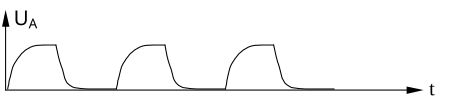
\includegraphics[width=.8\linewidth]{media/abb-22}
  \caption{Diagramm Taktgeber}
\end{figure}

Betrachtet man das Oszilloskopbild dieser Schaltung (s. Abb. 21), so fällt auf, dass bei den Übergängen der beiden Bereiche keine genaue senkrechten Flanken entstehen. Dies spielt jedoch bei einer digitalen Schaltung keine Rolle. Die Impulslänge kann nun durch die Drehwiderstände verändert werden. Die genaue Dauer des Impulses und der Taktlücke lässt sich durch die Gleichung t=R·C bestimmen. \index{Oszilloskopbild}

Bei R=3k und C=100 nF erhält man also einen Impuls von t=3·10\textsuperscript{-4} s.

Einen besseren AMV (astabilen Multivibrator) zeigt Abb. 22. Das Herzstück dieser Schaltung ist der Präzisionstimer NE 555, der verhältnismäßig günstig ist. Der Vorteil des Timers ist vor allem die erhöhte Frequenzgenauigkeit und die genauere Impulsform der Rechteckspannung. Dies ist deutlich am Oszilloskopbild zu erkennen. Außerdem ist die Ausgangsleistung mit etwa 200 mA deutlich höher als bei der vorherigen Schaltung. Die Impulslänge kann durch Wahl der Widerstände und des Kondensators zwischen einigen ns und mehreren Sekunden (50 s und mehr) variiert werden.\index{Multivibrator}

\begin{figure}[htbp]
  \centering
  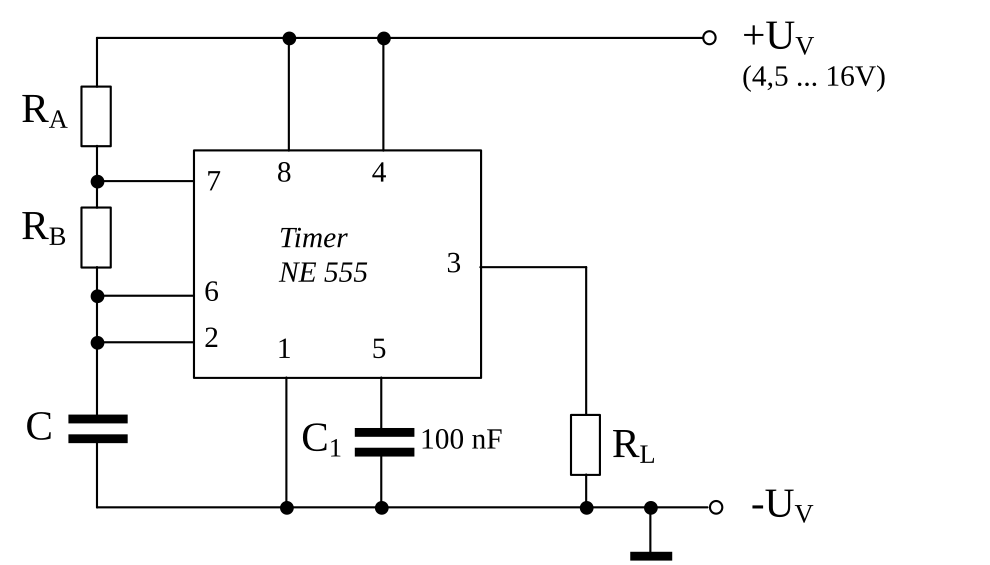
\includegraphics[width=.8\linewidth]{media/abb-23}
  \caption{Schaltbild Taktgeber mit einem NE555}
\end{figure}

\begin{figure}[htbp]
  \centering
  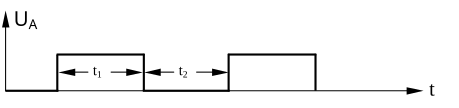
\includegraphics[width=.8\linewidth]{media/abb-24}
  \caption{Diagramm Zeitverhalten NE555}
\end{figure}

\begin{quote}
  t\textsubscript{1} = 0,7(R\textsubscript{A}+R\textsubscript{B})·C
\end{quote}


\begin{quote}
  t\textsubscript{2} = 0,7·R\textsubscript{B}·C
\end{quote}


\begin{quote}
  t\textsubscript{1}+t\textsubscript{2} = 0,7(R\textsubscript{A}+2R\textsubscript{B})·C
\end{quote}


Nun kann es jedoch manchmal auch nötig sein, einzelne Impulse, die von Hand ausgelöst werden, an eine digitale Schaltung zu legen. Dies ist vor allem von großem Nutzen, wenn die Schaltung nach jedem Schritt kontrolliert werden soll. Nun könnte man einfach einen Taster nehmen, mit der Stromversorgung verbinden und durch das Drücken der Taste einen Impuls erzeugen. Doch leider geht das nicht so einfach. Der Grund dafür ist in Abb. 24 zu erkennen.

\begin{figure}[htbp]
  \centering
  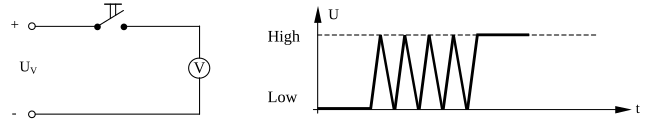
\includegraphics[width=.8\linewidth]{media/abb-25}
  \caption{Diagramm Tastenprellen}
\end{figure}

Bei einem einfachen Taster ist eben keinesfalls beim Drücken der Taste sofort die angelegte Spannung am Ausgang vorhanden. Vielmehr „pendelt“ der Spannungswert zwischen High und Low viele Male hin und her bevor der Spannungswert konstant bleibt. Das geschieht zwar mit einer sehr hohen Frequenz, doch sind gerade digitale Schaltungen auf sehr hohe Frequenzen (im Megahertz bis Gigahertz-Bereich) ausgelegt und reagieren damit auf diese schnellen Wechsel. Falls also ein einfacher Taster verwendet wird, ist eine sog. „Entprellung“ unbedingt erforderlich. Den Schaltplan dazu zeigt Abb. 25. Wie man sieht, ist auch diese Schaltung mit Standard-Gattern aufgebaut, nämlich zwei NAND-Gattern.\index{Spannung}\index{Spannungswert}

\begin{figure}[htbp]
  \centering
  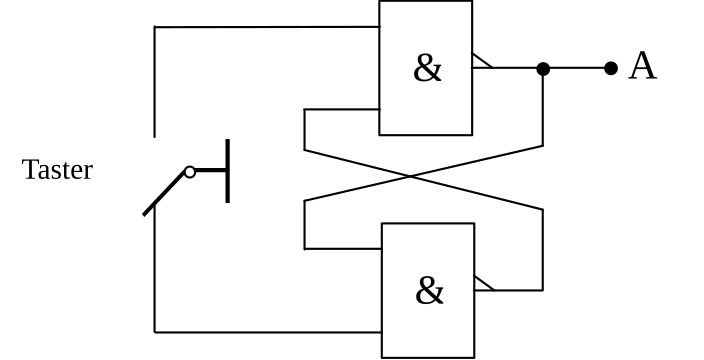
\includegraphics[width=.8\linewidth]{media/abb-26}
  \caption{Schaltbild verhinderung Tastenprellen}
\end{figure}

Eine weitaus bessere Schaltung für Einzelimpulse ist in Abb. 26 dargestellt. Dabei findet wieder der Timer-IC NE 555 von Texas Instruments Verwendung. Man kann nun durch die Wahl des Widerstandes R und des Kondensators C die Impulsdauer bestimmen und zwar von einigen ns bis zu mehreren Sekunden. Bei der einfachen entprellten Taste kann man zwar auch durch mehr oder weniger langes Drücken der Taste die Impulsdauer grob bestimmen, doch versagt diese Methode bei kurzen Einschaltzeiten. Außerdem ist auch hier der Ausgang höher belastbar.

\begin{figure}[htbp]
  \centering
  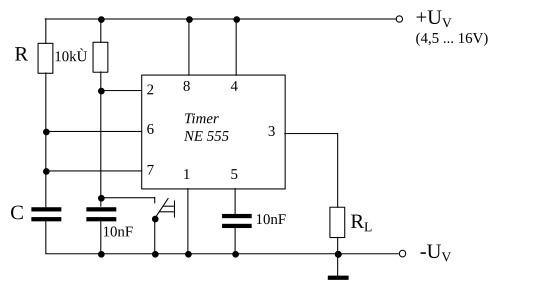
\includegraphics[width=.8\linewidth]{media/abb-27}
  \caption{Schaltbild eines Einzelimpulsgebers}
\end{figure}

\begin{figure}[htbp]
  \centering
  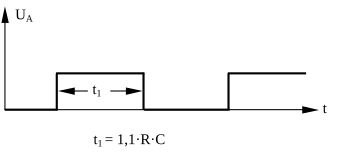
\includegraphics[width=.8\linewidth]{media/abb-28}
  \caption{Diagramm Einzelimpulsgebers}
\end{figure}

\section{Taktgeber allgemein}

Der Takt, und somit der Taktgeber, spielen in der Digitaltechnik eine sehr große Rolle. Zum Beispiel in einer Digitaluhr, einem Zählwerk oder einem Computer.\index{Taktgeber}

Um nun aber nicht immer einen kompletten Taktgeber in einer Schaltung zeichnen zu müssen, hat man auch dafür ein Schaltsymbol. Abb. 28 zeigt dies mit einer kleinen Raffinesse. Wenn man nämlich an den Ausgang ein AND-Gatter schaltet und den anderen Eingang des AND-Gatters in der angegebenen Weise mit einem Takter, der an L liegt verbindet, kann die Zeit, in der die Impulse am Ausgang A liegen bestimmt werden. Impulse gelangen nur dann zum Ausgang A, wenn der Taster gedrückt ist. Vorteilhaft ist dies vor allem bei sehr kurzer Impulsdauer.\index{Taktgeber}\index{AND}\index{Gatter}

Der H-Wert kann auch bei umfangreicheren Schaltungen auf andere Weise an den unteren Eingang des AND-Gatters gelangen. Zum Beispiel durch eine weitere Verknüpfungsschaltung die dann den Wert L liefert, wenn ein Zähler einen bestimmten Stand erreicht hat. In diesem Fall sperrt das AND-Gatter den Impuls durch einen L-Wert am unteren Eingang und der Zähler kann durch das Ausbleiben von Impulsen nicht mehr weiterzählen.\index{AND}\index{Gatter}

\begin{figure}[htbp]
  \centering
  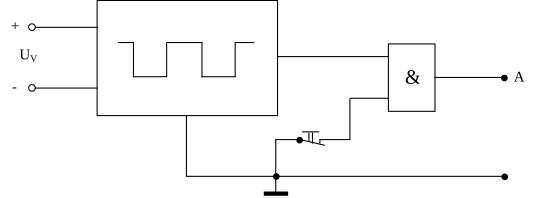
\includegraphics[width=.8\linewidth]{media/abb-29}
  \caption{Abschaltbarer Taktgeber}
\end{figure}


\chapter{Flipflops}

\section{R-S-Flipflop (Setzspeicher)}

Dieses Bauteil ist das einfachste Speicherglied der Digitaltechnik. Es kann einen bestimmten Wert über eine gewisse Zeit speichern. Am besten lässt sich das Verhalten an der NAND-Schaltung erklären. Allerdings ist diese Schaltung nur eine Prinzipschaltung, die z.B. nicht das „Warum“ der Speicherung erklärt.

\begin{figure}[htbp]
  \centering
  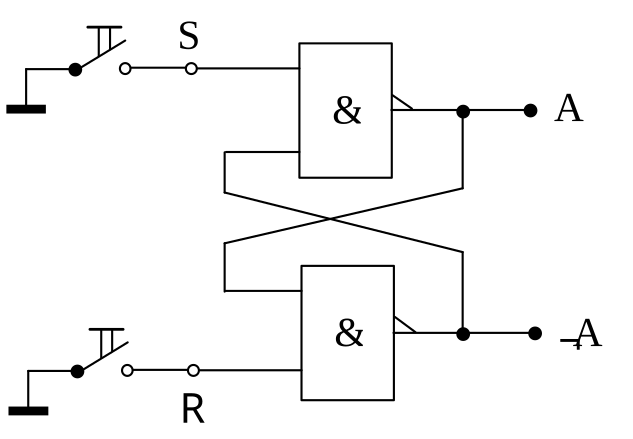
\includegraphics[width=.8\linewidth]{media/abb-30}
  \caption{Schaltbild RS-FlipFlop}
\end{figure}

Setzt man in dieser Schaltung den S-Eingang („Setz-Eingang“) mit dem Taster auf 0, so hat der Ausgang A den Wert 1. Wird dagegen der untere Taster betätigt und somit der R-Eingang („Rücksetz-Eingang“) auf den Wert 0 gelegt, so erscheint am Ausgang A der Wert 0. Der komplementäre Ausgang \ensuremath{\lnot}A hat immer den entgegengesetzten Wert von A. Das Wesentliche dieser Schaltung ist aber, dass durch Betätigen von z.B. Taster S der Wert 1 am Ausgang „gespeichert“ bleibt – auch nach dem Loslassen der Taste. Und zwar so lange, bis durch Betätigen des Tasters R der Ausgang auf den Wert 0 gesetzt wird. Dabei spielt es keine Rolle, ob der Taster bei S noch gedrückt ist oder nicht. Abb. 30 verdeutlicht das Verhalten der Schaltung. Abb. 31 zeigt das Schaltsymbol für RS-Flipflops.

\begin{figure}[htbp]
  \centering
  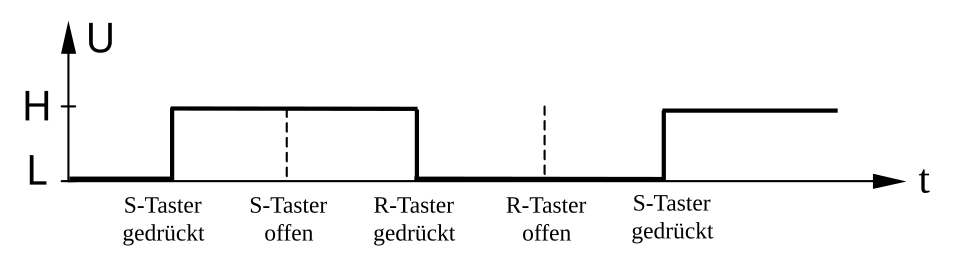
\includegraphics[width=.8\linewidth]{media/abb-31}
  \caption{Diagramm RS-FlipFlop}
\end{figure}

\begin{figure}[htbp]
  \centering
  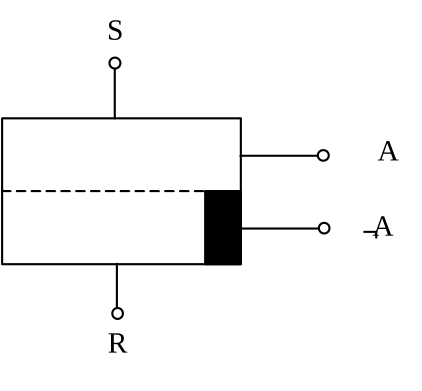
\includegraphics[width=.8\linewidth]{media/abb-32}
  \caption{Schaltsymbol RS-FlipFlop}
\end{figure}

Den Setzspeicher findet man als IC meist nicht als einzelne Schaltung. Vielmehr haben andere Flipflops wie z.B. das JK-Flipflop das RS-Flipflop integriert. Durch geeignete Beschaltung ist es aber nicht schwer, solch ein Flipflop als RS-Flipflop zu betreiben. In manchen Datenbüchern und Applikationen sind die beiden Eingänge mit \ensuremath{\lnot}R und \ensuremath{\lnot}S bezeichnet. Das bedeutet nichts anderes, als eine Unterstreichung der Tatsache, dass z.B. das Setzen nicht durch S=1 sondern durch S=0 erfolgt. Und das ist ja nichts anderes als \ensuremath{\lnot}S=1.\index{JK-Flipflop}

Um nun in einem Übungsaufbau den Wert am Ausgang sofort zu erkennen, empfiehlt es sich, eine Leuchtdiode (LED) dazuzuschalten. Leuchtet sie, so hat der Ausgang den Wert 1. Der komplementäre Ausgang \ensuremath{\lnot}A hat somit den Wert 0. Ist die LED dunkel, so hat A den Wert 0 und \ensuremath{\lnot}A den Wert 1.\index{LED}

\section{Das JK-Flipflop (Master-Slave-Flipflop)}

Ein weiteres und sehr wichtiges Flipflop ist das JK-Flipflop. Mit ihm können viele Zähler und Teiler aufgebaut werden. Wie man an dem Schaltsymbol erkennt, hat auch dieses Flipflop einen Setz- und einen Rücksetzeingang. Werden diese beiden Anschlüsse verwendet, so kann man das Bauteil als gewöhnliches RS-Flipflop betreiben. Dazu sollten aber die anderen Eingänge nicht angeschlossen sein um eine Fehlschaltung am Ausgang zu vermeiden.\index{JK-Flipflop}\index{Rücksetzeingang}

Das JK-Flipflop kann alternativ dazu über die beiden Eingänge J und K betrieben werden. Für diesen Fall besitzt es noch einen weiteren Eingang T, über den dem Flipflop ein Taktimpuls zugeführt werden kann.\index{JK-Flipflop}\index{Taktimpuls}

Prinzipiell unterscheidet man zwei Arten von JK-Flipflops: Das „positiv-flankengetriggerte“ und das „negativ-flankengetriggerte“. Beim positiv-flankengetriggerten Flipflop, das in Abb. 32 dargestellt ist, erfolgt die Schaltung am Ausgang durch den ansteigenden Teil des angelegten Takt-Impulses. Das bedeutet, dass die Werte am Ausgang, die durch J und K bestimmt werden mit dem Ansteigen des Taktimpulses von L auf H ihren Wert ändern. Dargestellt ist das im Schaltsymbol durch die ansteigende Flanke eines Rechteckimpulses in der oberen rechten Ecke des Schaltsymbols. 

\begin{figure}[htbp]
  \centering
  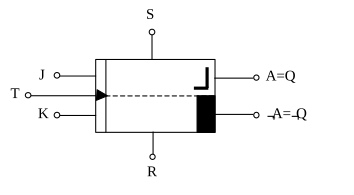
\includegraphics[width=.8\linewidth]{media/abb-33}
  \caption{Schaltsymbol JK-FlipFlop (positive Flanke)}
\end{figure}

Beim negativ-flankengetriggerten JK-Flipflop, das in der Technik hauptsächlich verwendet wird, erfolgt die Umschaltung beim Abfallen des Impulses von H auf L. Abb. 33 symbolisiert ein solches Bauteil. Das Unterscheidungsmerkmal gegenüber dem vorherigen Flipflop ist die abfallende Flanke eines Rechteckimpulses.\index{JK-Flipflop}

\begin{figure}[htbp]
  \centering
  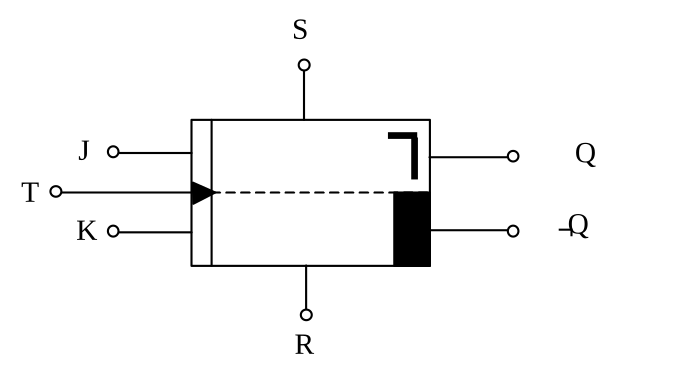
\includegraphics[width=.8\linewidth]{media/abb-34}
  \caption{Schaltsymbol JK-FlipFlop (negative Flanke)}
\end{figure}

Wohlbemerkt sind die beiden Eingänge R und S in diesem Fall nicht angeschlossen. Sie haben nämlich Priorität, d.h. sie sind vom Takt unabhängig. Doch dazu später mehr.

Wie schon bei der Unterscheidung der beiden JK-Flipflops erwähnt wurde, ist ein Taktimpuls bei diesem Bauteil sehr wichtig. Angelegt wird er am Eingang T. Von ihm hängt es z.B. ab, wie schnell sich ein Wert am Ausgang Q oder \ensuremath{\lnot}Q ändern kann. Die Logik-Tafel gibt über die Werte am Ausgang genauer Auskunft.\index{Taktimpuls}

\begin{table}[htbp]
  \centering
  \begin{tabular}{cccc}
    \toprule
    J & K & Q & \ensuremath{\lnot}Q \\
    \midrule
    0 & 1 & 0 & 1 \\
    1 & 0 & 1 & 0 \\
    0 & 0 & Q & \ensuremath{\lnot}Q \\
    1 & 1 & \ensuremath{\lnot}Q & Q \\
    \bottomrule
  \end{tabular}
\end{table}

Hat der J-Eingang den Wert 0 und K den Wert 1, so liegt am Ausgang Q der Wert 0. Entsprechend hat der komplementäre Ausgang \ensuremath{\lnot}Q den Wert 1.

Wechselt nun der J-Eingang auf den Wert 1 und der K-Eingang auf den Wert 0, so hat der Ausgang Q den Wert 1 und \ensuremath{\lnot}Q den Wert 0.

Wenn beide Eingänge den Wert 0 haben, so ändert sich das Ausgangssignal nicht, das bedeutet, dass der vorherige Wert des Ausgangs beibehalten wird.\index{Ausgangssignal}

Falls beide Eingänge den Wert 1 aufweisen, so dreht sich das Ausgangssignal gerade um. Sowohl Q als auch \ensuremath{\lnot}Q nehmen jeweils ihren komplementären Wert an. Oder anders ausgedrückt: Q nimmt den Wert von \ensuremath{\lnot}Q an und \ensuremath{\lnot}Q den Wert von Q.\index{Ausgangssignal}

Allerdings kann sich das Ausgangssignal nur ändern, wenn ein Taktimpuls wirksam geworden ist. Um also ein Umschalten des Wertes am Ausgang zu erreichen, muss unbedingt ein Takt angelegt werden. Sobald nun bei einem negativ-flankengetriggerten Flipflop eine negative Flanke an T anliegt, stellen sich die Ausgänge Q und \ensuremath{\lnot}Q entsprechend den Eingängen J und K um.\index{Ausgangssignal}\index{Taktimpuls}

Die Eingänge R und S sind dagegen vom Taktimpuls unabhängig. Sobald z.B. der Setzeingang auf Masse gelegt wird, erscheint am Ausgang der Wert 1, auch dann, wenn gerade kein Taktimpuls wirksam wurde. Ebenso funktioniert die Schaltung wenn der Rücksetzeingang R mit Masse verbunden wird. Dann erscheint am Ausgang A der Wert 0. Sobald der R- oder der S-Eingang benutzt wird, ist die übrige Beschaltung (also T, J und K) nicht wirksam.\index{Taktimpuls}\index{Rücksetzeingang}

In Abb. 34 ist nun das Schaltverhalten eines negativ-flankengetriggerten Flipflops dargestellt. Deutlich zu sehen ist dabei, dass ein Umschalten des Signals am Ausgang nur dann erfolgen kann, wenn der Taktimpuls T gerade abfällt.\index{Taktimpuls}

Spannungs-Diagramm (Schaltdiagramm) für ein negativ-flankengetriggertes JK-Flipflop:\index{JK-Flipflop}

\begin{figure}[htbp]
  \centering
  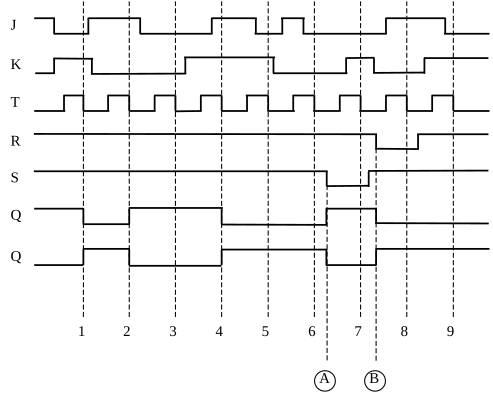
\includegraphics[width=.8\linewidth]{media/abb-35}
  \caption{Diagramm Zeitverhalten JK-FlipFlop}
\end{figure}

Zur Verdeutlichung hier nun die Erläuterung:

J=0, K=1. Da R und S den Wert 1 haben, also nicht wirksam sind, kann der Takt wirksam werden. In der Logik-Tafel sieht man, dass der Ausgang Q den Wert 0 haben muss. Deshalb nimmt Q auch im Diagramm beim Abfallen der Taktflanke T den Wert 0 an.

J=1, K=0. Damit hat Q den Wert 1.

J=K=0. Am Ausgang Q erscheint der Wert 1, da laut Logik-Tafel der Wert gleich bleibt.

J=K=1. Nun erscheint am Ausgang das gegenteilige Signal, das zuvor an Q lag. In diesem Fall ist es der Wert 0.

J=0, K=1. Damit hat der Ausgang Q den Wert 0.

J=K=0. Das Signal am Ausgang bleibt gleich, also auf 0.

Bei Punkt A wird nun der Setzeingang S auf Masse gelegt. Damit nimmt der Ausgang Q sofort den Wert 1 an. Dies geschieht wie man sieht auch ohne Taktimpuls.\index{Taktimpuls}

Der Setzeingang S liegt noch immer auf Masse. Somit sind die Signale von J und K nicht wirksam, wenngleich auch eine negative Taktflanke vorliegt.

Im Punkt B ist nun der Setzeingang S wieder auf dem Wert 1. Dagegen wird der Rücksetzeingang R auf Masse, also auf den Wert 0 gelegt. Damit nimmt der Ausgang Q sofort den Wert 0 an.\index{Rücksetzeingang}

R ist noch immer auf Masse gelegt. Damit hat der Ausgang unabhängig von J und K den Wert 0.

J=0, K=1. R hat nun wieder den Wert 1, ist also genau wie S nicht wirksam. Der Taktimpuls kann also wieder wirksam werden und schaltet deshalb bei der abfallenden Taktflanke den Ausgang Q auf den Wert 0.\index{Taktimpuls}

Zu bemerken wäre noch, dass bei nicht wirksamen Eingängen R und S zwischen den einzelnen Takt-Impulsen die Eingänge J und K jeden beliebigen Wert annehmen können ohne dass sich der Wert am Ausgang Q verändert. Sie können auch ihren Wert zwischen zwei Impulsen mehrmals wechseln. Für das Umschalten am Ausgang ist nur interessant, was zur Zeit der abfallenden Taktflanke für Signale an J und K liegen. Nur nach diesen Werten richtet sich der Wert des Ausgangs Q.

Abb. 35 zeigt die Innenschaltung des JK-Flipflops. Das Master-Slave-Flipflop besteht intern aus 2 bistabilen Multivibratoren mit gesteuerter Übernahme, die in Reihe (hintereinander) geschaltet sind. Der sogenannte Master (engl. Master = Herr, Meister) besteht aus den Verknüpfungsschaltungen V3 und V4. Die NAND-Gatter V1 und V2 bilden die dazugehörige Torschaltung. Die J- und K-Eingänge sind UND-verknüpft. Die Verknüpfungsschaltungen V5 und V6 bilden die Torschaltung des Slave (engl. Slave = Knecht, Sklave). Der Multivibrator des Slave besteht aus den Verknüpfungsschaltungen V7 und V8. Der Multivibrator verfügt noch über 2 Eingänge, die nicht über die Torschaltung laufen, also auch unabhängig vom Takt wirksam sind: L-Pegel am Setzeingang S stellt den Ausgang Q auf den Wert 1, L-Pegel am Rücksetzeingang R stellt Q wieder auf den Wert 0 zurück.\index{Verknüpfungsschaltungen}\index{Gatter}\index{Multivibrator}\index{Rücksetzeingang}

\begin{figure}[htbp]
  \centering
  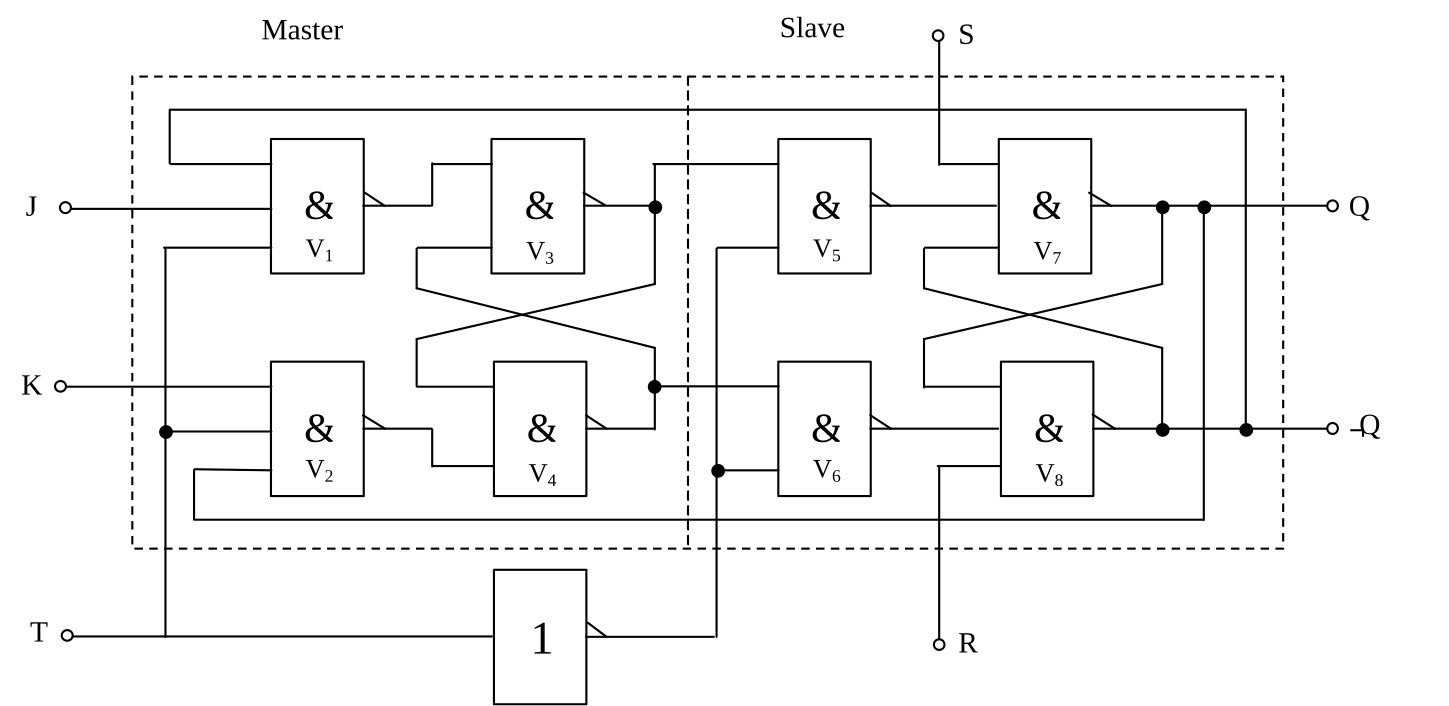
\includegraphics[width=.8\linewidth]{media/abb-36}
  \caption{Schaltbild Master-Slave-Flipflop}
\end{figure}

\section{Dualzähler}

Aus dem JK-Flipflop lässt sich nun eine in der Technik oft gebrauchte Zählerschaltung realisieren. Dabei werden oft die Eingänge S und R neben den J- und K-Eingängen benutzt. Der Einfachheit halber werden hier nur die J- und K-Eingänge sowie der R-Eingang verwendet. Natürlich wird auch der Takteingang T angeschlossen.\index{JK-Flipflop}\index{Takteingang}

Wenn man an ein JK-Flipflop einen Takt T anlegt, so hat der Ausgang Q\textsubscript{0} bei jeder negativen Taktflanke eine Wertänderung, also einen dauernden Wechsel zwischen 1 und 0. Abb. 37 zeigt den zeitlichen Verlauf des Ausgangs Q\textsubscript{0} in Abhängigkeit vom angelegten Takt T. Jetzt wird an das zweite JK-Flipflop das Ausgangssignal Q\textsubscript{0} angeschlossen. Somit bestimmt der Ausgang des ersten Flipflops den Takt des zweiten Flipflops. Das Anschlussbild ist in Abb. 36 zu sehen.\index{JK-Flipflop}\index{Ausgangssignal}

Wie man im Spannungsdiagramm der Schaltung erkennt, hat der Ausgang Q\textsubscript{1} die halbe Taktfrequenz wie Q\textsubscript{0}. Dies beruht wiederum darauf, dass eine Umschaltung des Flipflops nur bei einer negativen Taktflanke stattfindet. Die Schaltzustände der beiden Flipflops entsprechen, wie unter dem Diagramm aufgezählt, dem dualen Zählerstand. Der Zähler kann also nur bis zur Zahl 11 des Dualsystems zählen. Das entspricht der dezimalen Zahl 3. Danach kehrt er automatisch wieder zur Anfangszahl 00 zurück.\index{Taktfrequenz}\index{Dualsystems}

\begin{figure}[htbp]
  \centering
  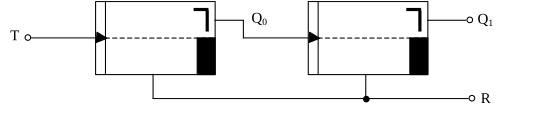
\includegraphics[width=.8\linewidth]{media/abb-37}
  \caption{Schaltbild Dualzähler}
\end{figure}

Wenn nun der Rücksetzeingang R, der oftmals auch Reset-Eingang genannt wird, auf Masse gelegt wird, erscheint auf jeden Fall der Wert 0 an beiden Ausgängen. Dabei ist der Takt nicht von Bedeutung, ebenso die Schaltzustände der beiden Ausgänge Q\textsubscript{0} und Q\textsubscript{1}. Im folgenden Diagramm wird kurz nach dem zweiten Erscheinen der Zahl 11 (dual) der Reset-Eingang aktiviert. Man sieht, dass die beiden Ausgänge sofort den Wert 0 annehmen, obwohl keine negative Flanke vorliegt. Das wurde ja bereits im letzten Abschnitt näher erläutert. Dieser Sachverhalt wird nun bei Zählern angewandt, die bis zu einer bestimmten Zahl zählen sollen, die durch eine einfache Aneinanderreihung von Flipflops nicht erreicht wird. Beispielsweise könnte man mit der in Abb. 36 dargestellten Schaltung einen Zähler bauen, der nach der Zahl 2, also dual 10, auf 0 zurückspringt. Genaueres darüber wird im nächsten Abschnitt behandelt.\index{Rücksetzeingang}

\begin{figure}[htbp]
  \centering
  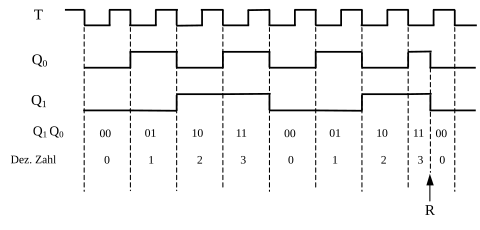
\includegraphics[width=.8\linewidth]{media/abb-38}
  \caption{Diagramm Dualzähler}
\end{figure}

\section{Dualzähler für beliebige Zahlenreihen}

Der Dualzähler des vorherigen Abschnittes konnte nur Dualzahlen eines bestimmten Grades durchzählen. Beispielsweise von 00 bis 11 (entspricht dez. 3) oder bei einer Erweiterung der Schaltung durch zwei weitere JK-Flipflops von 0000 bis 1111 (entspricht dez. 15). Abhilfe gibt es dabei nur durch die Rücksetzung von Hand, das bedeutet den Rücksetzeingang R mit Hilfe eines Schalters auf Masse zu legen. Durch geeignete Verwendung der besprochenen Verknüpfungsschaltungen lässt sich nun der Rücksetzvorgang automatisch bewerkstelligen. Man muss nur die geeigneten Gatter zusammenschalten, die zu einem bestimmten Zeitpunkt den Zähler wieder auf Null zurücksetzt. Bei Zählern mit zwei oder drei JK-Flipflops ist das kein Problem. Selbst bei umfangreicheren Zählern gibt es leichte, sofort durchschaubare Rückstellschaltungen.\index{Rücksetzeingang}\index{Verknüpfungsschaltungen}\index{Gatter}

Als Beispiel wählen wir einen Zähler, der durch drei Flipflops aufgebaut ist. Das Schaltbild ist in Abb. 38 dargestellt. Dieser Zähler hat jedoch eine automatische Rückstellung bei der Zahl 110. Dies entspricht der dezimalen Zahl 6. 

\begin{figure}[htbp]
  \centering
  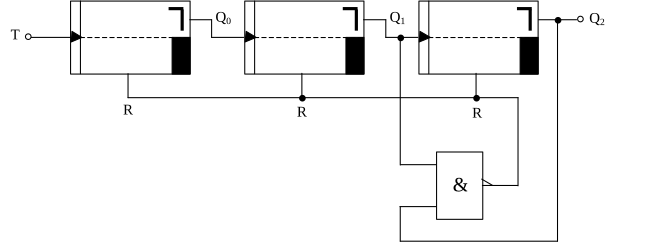
\includegraphics[width=.8\linewidth]{media/abb-39}
  \caption{Schaltbild Binärzähler}
\end{figure}

\begin{figure}[htbp]
  \centering
  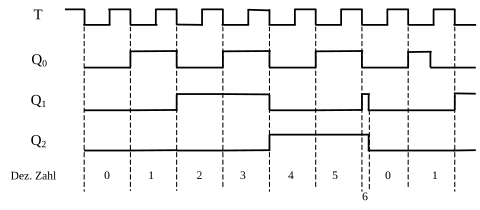
\includegraphics[width=.8\linewidth]{media/abb-40}
  \caption{Diagramm Binärzähler}
\end{figure}

Wichtig ist die Zahl 6 in diesem Zähler nur für die Rückstellung. In Abb. 39 wurde die Zeitspanne für die Zahl 6 zur besseren Verständlichkeit übertrieben dargestellt. Tatsächlich erscheint diese Zahl so kurz, dass sie für den Zählvorgang keine Bedeutung hat. Es handelt sich hier also um einen Zähler von 0 bis 5. Diese Reihe wird ganz normal durchlaufen. Sobald aber der Zähler am Ausgang Q\textsubscript{1} und Q\textsubscript{2} gleichzeitig den Wert 1 hat, wird durch das NAND-Gatter der Reset-Eingang aller JK-Flipflops auf 0 gelegt. Der Zähler beginnt erneut von 0 an zu zählen.\index{Gatter}

Es ist also wichtig, dass bei einem beliebigen Zähler der Rücksetzvorgang mit der nächsthöheren Ziffer des eigentlichen Zählumfangs aktiviert wird. Wenn z.B. ein Zähler bis 18 zählen soll, so muss der Rücksetzeingang durch eine geeignete Verknüpfungsschaltung für die Zahl 19 auf den Wert 0 gelegt werden.\index{Rücksetzeingang}

Der Rücksetzeingang bleibt nun so lange auf dem Wert 0, wie in unserem Beispiel Q\textsubscript{1} und Q\textsubscript{2} den Wert 1 haben. Da aber in wenigen ns der Rücksetzvorgang beendet ist (R hat Priorität), kann die nächste negative Taktflanke für das Umschalten des ersten Flipflops wirksam werden. Somit erscheint nach der dezimalen Zahl 0 (durch den Rücksetzvorgang) im nächsten Takt die 1. Problematisch wird diese Art der Rücksetzung nur bei sehr hohen Taktfrequenzen, oder bei sehr empfindlichen Schaltungen, die bei diesem kurzen Erscheinen der höheren Zahl „umkippen“ können. In diesem Fall muss man sich mit einer anderen Art der Rücksetzung behelfen. Meist genügt jedoch diese Art der Rückstellung. Die Impulsdauer sollte jedoch bei TTL-Schaltungen nicht unter 18 ns liegen, da diese Zeit zum Umschalten benötigt wird.\index{Rücksetzeingang}

\section{D-Flipflop (Datenspeicher)}

Das D-Flipflop ist ein einfaches Datenspeicherglied. Es kann einen bestimmten Wert abhängig vom Takt T und den Eingängen R und S speichern. Dabei haben die beiden letztgenannten Eingänge wie auch beim JK-Flipflop Priorität. Das bedeutet, dass das Flipflop unabhängig vom Takt einen gewünschten Wert annehmen kann, falls der Setz- bzw. Rücksetzeingang aktiviert wird. Sind diese beiden Eingänge jedoch auf den Wert 1 gesetzt (also nicht aktiv), so erfolgt bei jeder negativen Takt-Flanke eine Übernahme des Dateneingangs D an den Ausgang Q. Der komplementäre Ausgang \ensuremath{\lnot}Q hat auch hier wieder den entgegengesetzten Wert von Q. Das Verhalten von D in Abhängigkeit vom Takt T und den Eingängen S und R zeigt das abgebildete Spannungsdiagramm. \index{JK-Flipflop}\index{Rücksetzeingang}

Die Industrie bietet D-Flipflops schon fertig aufgebaut als ICs an. Haben Sie diese jedoch nicht zur Hand, so kann man mit Hilfe eines JK-Flipflops einen solchen Datenspeicher aufbauen. Dazu ist es notwendig den K-Eingang über einen Inverter an den J-Eingang anzuschließen. An K liegt also \ensuremath{\lnot}J. Wird nun an J der Wert der gewünschten Daten gelegt, so übernimmt das Flipflop bei der nächsten negativen Taktflanke diesen Wert auf den Ausgang Q. Ist z.B. das Flipflop auf dem Wert Q=0 und hat der Dateneingang den Wert D=1, so wechselt nach einer negativen Taktflanke der Ausgang Q seinen Wert von 0 auf 1. Dieser Wert wird so lange gespeichert, bis über den Takt T und einen neuen Wert an D der Zustand von Q geändert wird. Natürlich wäre eine Änderung auch durch eine Aktivierung von S oder R möglich.\index{Dateneingang}

\begin{figure}[htbp]
  \centering
  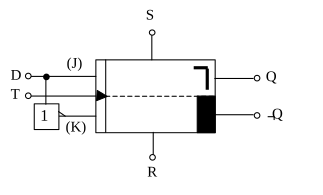
\includegraphics[width=.8\linewidth]{media/abb-41}
  \caption{Schaltbild D-FlipFlop}
\end{figure}

\begin{figure}[htbp]
  \centering
  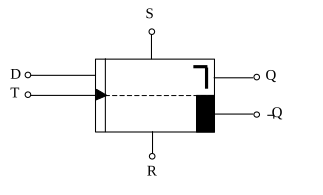
\includegraphics[width=.8\linewidth]{media/abb-42}
  \caption{Schaltsymbol D-FlipFlop}
\end{figure}

\begin{figure}[htbp]
  \centering
  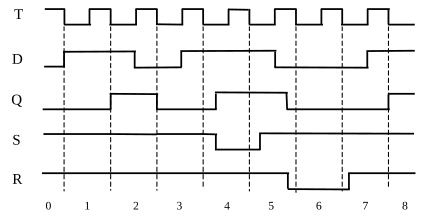
\includegraphics[width=.8\linewidth]{media/abb-43}
  \caption{Diagramm D-FlipFlop}
\end{figure}

Ein wichtiges Anwendungsbeispiel eines D-Flipflops ist das Schieberegister. Dieses Bauteil ist in einem eigenen Kapitel noch genauer erklärt.


\chapter{KV-Tafel}

\section{Einführung}

Um bei komplizierten Rücksetzbedingungen oder bei Ansteuerungen von LEDs und Siebensegmentanzeigen eine möglichst einfache Kombination von Verknüpfungsschaltungen zu erreichen, bedient man sich meist der sogenannten KV-Tafeln. Es ist eine systematische Methode bei der ein bestimmtes Schema die Erkennung der benötigten Verknüpfungsschaltungen erleichtert. Entwickelt wurde es von Karnaugh und Veitch. Bei dem Verfahren werden die Variablen in rechteckigen Feldern der KV-Tafel dargestellt.\index{Verknüpfungsschaltungen}\index{KV-Tafeln}\index{Verknüpfungsschaltungen}

Ein Beispiel:

Der Ausgang A soll ein Segment einer 7-Segment-Anzeige ansteuern. Gewählt wurde das oberste waagerechte Segment. Dabei wählen wir den Zähler von vorher, der von 0 bis 5 zählt. Der Ausgang A muss bei 0, 2, 3 und 5 den Wert 1 haben, da bei diesen Zahlen das Segment leuchten muss.

\begin{table}[htbp]
  \centering
  \begin{tabular}{ccccc}
    \toprule
    Q\textsubscript{2} & Q\textsubscript{1} & Q\textsubscript{0} & A & Dez. Zahl \\
    \midrule
    0 & 0 & 0 & 1 & 0 \\
    0 & 0 & 1 & 0 & 1 \\
    0 & 1 & 0 & 1 & 2 \\
    0 & 1 & 1 & 1 & 3 \\
    1 & 0 & 0 & 0 & 4 \\
    1 & 0 & 1 & 1 & 5 \\
    \bottomrule
  \end{tabular}
\end{table}

Durch diese Logik-Tafel ist nun der Zusammenhang der Dualzahlen (Q\textsubscript{2}Q\textsubscript{1}Q\textsubscript{0}) und dem Anschluss A des Segments gegeben. Es soll eine Decoderschaltung gefunden werden, die das Segment nur bei den dafür bestimmten Zahlen zum Leuchten bringt.

Nun werden zuerst so viele quadratische Felder aufgezeichnet, wie der Zähler im Höchstfall erreichen kann. Das wäre in unserem Fall mit 3 JK-Flipflops die Ziffern 0 bis 7, also 8 Zahlen. Bei Zählern mit 4 Flipflops wären es 16 usw.

Danach werden die Felder in sich überlappende Bereiche unterteilt. Die komplementären Ausgänge \ensuremath{\lnot}Q\textsubscript{2}, \ensuremath{\lnot}Q\textsubscript{1}, \ensuremath{\lnot}Q\textsubscript{0} werden dabei ebenfalls berücksichtigt. Nun werden die Werte 1 für A in das Diagramm eingetragen. Die kleine Ziffer im rechten oberen Eck ist die dezimale Zahl dieses Feldes. Als Beispiel der Wert 1 für die dez. Zahl 0 (\ensuremath{\lnot}Q\textsubscript{0}, \ensuremath{\lnot}Q\textsubscript{1}, \ensuremath{\lnot}Q\textsubscript{2}) in die linke untere Ecke. Man nimmt immer die „Einserausgänge“ für die Bestimmung des Feldes. Bei der Zahl 000 des dualen Systems muss also jedes Mal der komplementäre Ausgang (\ensuremath{\lnot}Q\textsubscript{2}, \ensuremath{\lnot}Q\textsubscript{1}, \ensuremath{\lnot}Q\textsubscript{0}) genommen werden, da diese den Wert 1 haben. Somit wird die dezimale Zahl 0 in das obere rechte Eck des Feldes mit den Koordinaten \ensuremath{\lnot}Q\textsubscript{2}, \ensuremath{\lnot}Q\textsubscript{1}, \ensuremath{\lnot}Q\textsubscript{0} geschrieben und der Wert, den der Ausgang A bei dieser Zahl hat in dem Kästchen vermerkt. Bei der dualen Zahl 101 wäre also das Fach mit den Koordinaten Q\textsubscript{2}, \ensuremath{\lnot}Q\textsubscript{1}, Q\textsubscript{0} gemeint.

Mit diesem Schema wird nun das ganze Diagramm ausgefüllt. Die Felder, die danach noch frei sind, werden mit einem „Kreuz“ versehen, da sie ja beim Zählvorgang nicht vorkommen. Bei ihnen ist es also gleichgültig, ob sie nun den Wert 1 oder 0 haben.

Nun werden die „Einser“ in 2er oder 4er Gruppen zusammengefasst. Allerdings darf eine Zusammenfassung nicht diagonal erfolgen, wohl aber über den Rand hinweg. Die einzelnen Felder einer solchen Gruppe werden in der nachfolgenden mathematischen Gleichung durch ein „und“-Zeichen verknüpft. Die einzelnen Gruppen dagegen mit einem „oder“-Zeichen.

\begin{figure}[htbp]
  \centering
  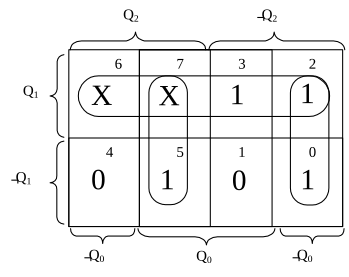
\includegraphics[width=.8\linewidth]{media/abb-44}
  \caption{KV-Tafel}
\end{figure}

Man erhält also nach Zusammenfassung der Felder und Gruppen die mathematische Gleichung der Form:

\begin{quote}
  A = Q\textsubscript{1} \ensuremath{\vee} (Q\textsubscript{2} \ensuremath{\wedge} Q\textsubscript{0}) \ensuremath{\vee} (\ensuremath{\lnot}Q\textsubscript{0} \ensuremath{\wedge} \ensuremath{\lnot}Q\textsubscript{2})
\end{quote}


Das Umsetzen einer solchen Formel in eine Decoderschaltung wurde ja bereits bei den Verknüpfungsschaltungen erläutert. Man hält sich dabei stur an die mathematische Formel, das heißt für ein „und“-Zeichen ein AND-Gatter und für ein „oder“-Zeichen ein OR-Gatter. Damit ergibt sich die unten abgebildete Decoderschaltung die das Segment steuert.\index{Verknüpfungsschaltungen}\index{AND}\index{Gatter}\index{OR-Gatter}

\begin{figure}[htbp]
  \centering
  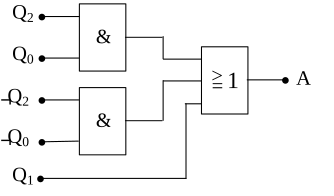
\includegraphics[width=.8\linewidth]{media/abb-45}
  \caption{Schaltbild Decoderschaltung}
\end{figure}

Der Einbau dieser Decoderschaltung erfolgt nun ganz analog. Es werden die benötigten Ausgänge der einzelnen Flipflops an die Schaltung angeschlossen und der Ausgang A an das Segment der 7-Segment-Anzeige.

\begin{figure}[htbp]
  \centering
  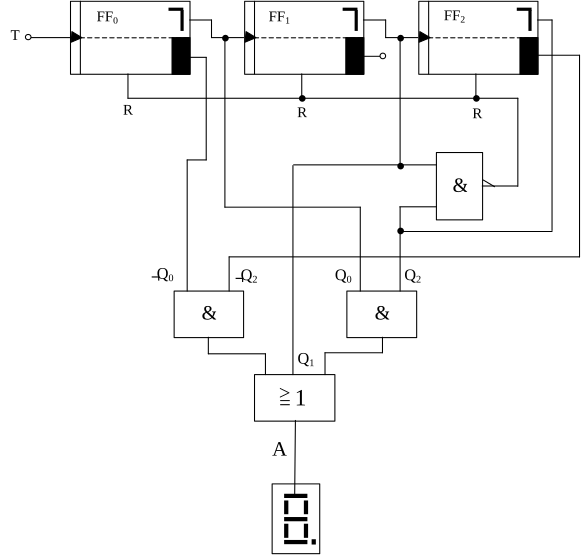
\includegraphics[width=.8\linewidth]{media/abb-46}
  \caption{Schaltbild Decoderschaltung}
\end{figure}

Dieses Verfahren erscheint auf den ersten Blick recht kompliziert, ist aber bei genau schematischer Durchführung sehr einfach und schnell auszuführen. Bei der rein mathematischen Darstellung würde ein umfangreiches Wissen der Algebra unbedingt nötig sein. Außerdem wäre der Überblick schwer zu behalten. Deshalb wählt man, wenn irgend möglich, diese Art der Lösung. Oftmals erkennt man auch sofort, wie die Decoderschaltung aussehen muss. Dann ist natürlich diese schematische Darstellung nicht nötig.

Ein weiteres Beispiel für die Anwendung der KV-Tafel. Ein Zähler, der von 0 bis 9 zählt, soll eine 7-Segment-Anzeige steuern. Gesucht ist nun die Decoderschaltung für das mittlere waagerechte Segment. Die Abhängigkeit des Ausganges A der Decoderschaltung, die das Segment ansteuert ist wiederum in der Tabelle aufgezeigt.

\begin{table}[htbp]
  \centering
  \begin{tabular}{cccccc}
    \toprule
    Q\textsubscript{3} & Q\textsubscript{2} & Q\textsubscript{1} & Q\textsubscript{0} & A & Dez. Zahl \\
    \midrule
    0 & 0 & 0 & 0 & 0 & 0 \\
    0 & 0 & 0 & 1 & 0 & 1 \\
    0 & 0 & 1 & 0 & 1 & 2 \\
    0 & 0 & 1 & 1 & 1 & 3 \\
    0 & 1 & 0 & 0 & 1 & 4 \\
    0 & 1 & 0 & 1 & 1 & 5 \\
    0 & 1 & 1 & 0 & 1 & 6 \\
    0 & 1 & 1 & 1 & 0 & 7 \\
    1 & 0 & 0 & 0 & 1 & 8 \\
    1 & 0 & 0 & 1 & 1 & 9 \\
    1 & 0 & 1 & 0 & X & 10 \\
    \bottomrule
  \end{tabular}
\end{table}

Die Rücksetzung geschieht bei Q\textsubscript{3} = Q\textsubscript{1} = 1. Diese beiden Ausgänge werden durch ein AND-Gatter miteinander verknüpft, negiert und an die Rücksetzeingänge der 4 JK-Flipflops angeschlossen. Man kann genauso gut ein NAND-Gatter nehmen anstatt des AND-Gatters und der nachfolgenden Negation.\index{AND}\index{Gatter}\index{NAND-Gatter}\index{Negation}

Die KV-Tafel muss nun 16 Felder haben, da insgesamt 16 Ziffern gezählt werden könnten (0 bis 15). Nun werden, genauso wie vorher die Felder in sich überlappende Zeilen und Spalten unterteilt. Dabei darf keine Zeile oder Spalte für zwei Ausgänge gleichzeitig gelten. Beispielsweise darf die erste und zweite waagerechte Spalte nicht gleichzeitig Q\textsubscript{0} und Q\textsubscript{2} sein, wohl darf eine Spalte Q\textsubscript{0}, die andere \ensuremath{\lnot}Q\textsubscript{0} sein, und gleichzeitig beide Spalten Q\textsubscript{2}.

Die einzelnen Felder werden nun genauso wie vorher ausgefüllt. Das bedeutet, dass zuerst die dezimalen Zahlen in die rechten oberen Ecken der Felder geschrieben werden. Dies geschieht, indem man die Ausgänge der Flipflops, die den Wert 1 haben zur Auffindung der Koordinaten zuhilfe nimmt. Beispielsweise soll das Feld für die duale Zahl 0100 (entspr. der dez. Zahl 4) aufgesucht werden. Q\textsubscript{3}, also die erste Ziffer, ist 0. Da aber ein 1-Wert benötigt wird, muss der invertierte Ausgang \ensuremath{\lnot}Q\textsubscript{3} genommen werden. Q\textsubscript{2} ist schon 1, deshalb ist der invertierte Ausgang nicht nötig. Q\textsubscript{1} und Q\textsubscript{0} sind wieder 0, daher wird auch hier der invertierte Ausgang verwendet. Nun liegen schon alle Koordinaten dieses Punktes fest. Er wird im KV-Diagramm aufgesucht und mit der Zahl 4 versehen.

Als weiteres Beispiel dient die duale Zahl 0101. Dabei sind die Ausgänge Q\textsubscript{3} und Q\textsubscript{1} Null. Also müssen hier die invertierten Ausgänge als Koordinaten verwendet werden. Q\textsubscript{2 }und Q\textsubscript{0} sind schon 1. Das ergibt die Feldkoordinaten \ensuremath{\lnot}Q\textsubscript{3}, Q\textsubscript{2}, \ensuremath{\lnot}Q\textsubscript{1}, Q\textsubscript{0}. Diese Koordinaten werden im KV-Diagramm aufgesucht und mit der Zahl 5 versehen.

Sind nun sämtliche Felder mit den dazugehörigen dezimalen Zahlen versehen, wird anhand der Tabelle der Wert A, der am Ausgang des Decoders erscheinen soll, in das dafür bestimmte Feld eingetragen. Für die Felder, die der Zähler durch die Rücksetzung nicht erreichen kann, wird ein „X“ eingetragen als Zeichen dafür, dass es gleichgültig ist, ob der Zähler in dieser Situation eine 0 oder 1 ausgibt.

\begin{figure}[htbp]
  \centering
  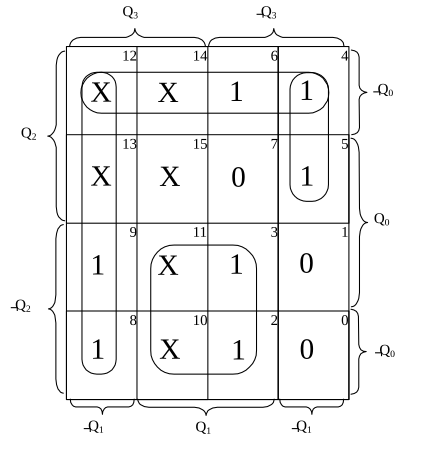
\includegraphics[width=.8\linewidth]{media/abb-47}
  \caption{KV-Tafel}
\end{figure}

Nun werden benachbarte Einser-Felder zu 2er oder 4er Gruppen zusammengefasst. Diese Zusammenfassung darf auch über den Rand hinaus und auf der anderen Seite weitergehen. Diagonal darf dagegen nicht zusammengefasst werden.

Die Koordinaten, die eine Gruppe gemeinsam hat, werden untereinander mit einem „und“-Zeichen der Booleschen Algebra zusammengefasst. Die Gruppen untereinander mit einem „oder“-Zeichen. Daraus ergibt sich die mathematische Formel:

\begin{quote}
  A = (\ensuremath{\lnot}Q\textsubscript{0} \ensuremath{\wedge} Q\textsubscript{2}) \ensuremath{\vee} (\ensuremath{\lnot}Q\textsubscript{1} \ensuremath{\wedge} Q\textsubscript{3}) \ensuremath{\vee} (Q\textsubscript{1} \ensuremath{\wedge} \ensuremath{\lnot}Q\textsubscript{2}) \ensuremath{\vee} (\ensuremath{\lnot}Q\textsubscript{1} \ensuremath{\wedge} Q\textsubscript{2} \ensuremath{\wedge} \ensuremath{\lnot}Q\textsubscript{3})
\end{quote}


Nun müssen nur noch die „und“-Gruppen, deren Ausgänge an ein AND-Gatter angeschlossen wurden, mit einem OR-Gatter verbunden werden. Damit ist der Decoder für das mittlere Segment der 7-Segment-Anzeige fertig.\index{AND}\index{Gatter}\index{OR-Gatter}

\begin{figure}[htbp]
  \centering
  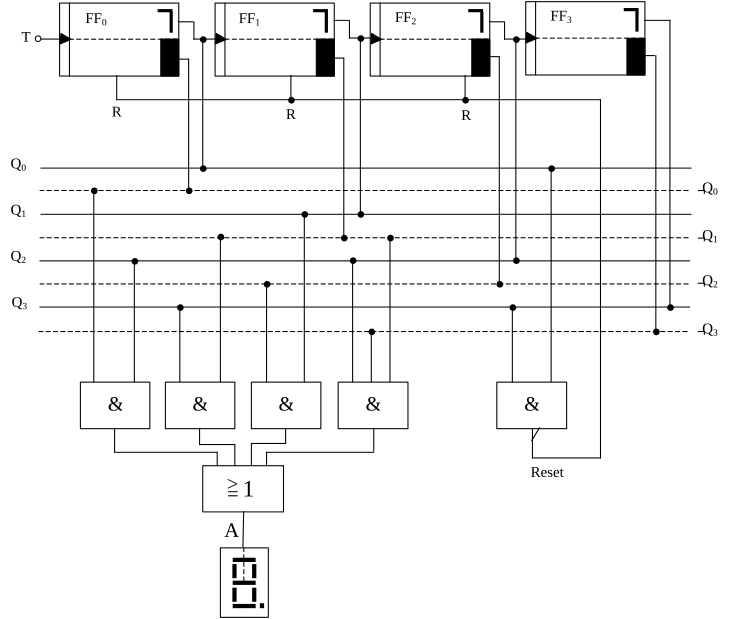
\includegraphics[width=.8\linewidth]{media/abb-48}
  \caption{Schaltbild Decoderschaltung}
\end{figure}


\chapter{Frequenzteiler}

\section{Einführung}

Für Digitaluhren, Frequenzmesser und viele weitere Schaltungen wird oft eine sehr genaue Zeitbasis verlangt. Das bedeutet, dass die Impulsdauer möglichst genau sein soll. Dies erreicht man am besten bei sehr hohen Frequenzen. Meist wird ein Quarz-Schwingkreis verwendet, der eine Schwingungszeit bis zu einigen MHz (Mega Hertz = 1 Mio. Hertz) und darüber hat. Doch können solche hohen Frequenzen nur sehr selten direkt verwendet werden. Vielmehr werden sie durch geeignete Frequenzteiler auf die benötigte Frequenz herunter gesetzt. So schwingt z.B. eine Quarzuhr mit der Frequenz 4194304 Hz. Durch Frequenzteilung wird daraus ein Impuls, der genau 1s dauert. Und diese Frequenz wird ja für eine Uhr gerade benötigt.

Der Aufbau des Teilers entspricht dem des Zählers. Die JK-Flipflops leisten uns auch hier wieder gute Dienste. Wie beim Zähler wird der Ausgang Q eines jeden Flipflops mit dem Takteingang des nächsten verbunden. Da nun eine Umschaltung am Ausgang nur durch eine negative Flanke des Eingangsimpulses erfolgen kann, wird der Eingangs-Impuls in jeder Stufe halbiert (geteilt).\index{Takteingang}

\begin{figure}[htbp]
  \centering
  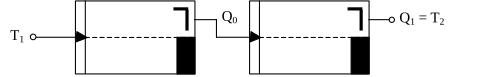
\includegraphics[width=.8\linewidth]{media/abb-49}
  \caption{Schaltbild Frequenzteiler}
\end{figure}

Der Sachverhalt der Frequenzteilung wird am Spannungsdiagramm besonders deutlich. Man sieht den Eingangsimpuls T, der von einem Taktgenerator (z.B. Quarzoszillator) geliefert wird. Darunter die beiden Ausgänge der Flipflops.

\begin{figure}[htbp]
  \centering
  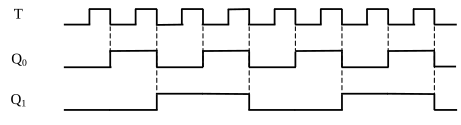
\includegraphics[width=.8\linewidth]{media/abb-50}
  \caption{Diagramm Frequenzteiler}
\end{figure}

Das Teilungsverhältnis dieser Schaltung ist 1:4, denn es sind 4 negative Taktflanken notwendig, um am Ausgang Q\textsubscript{1} eine negative Flanke auszulösen. Am Ausgang Q\textsubscript{0} wird eine Teilung 1:2 erreicht. Durch Hinzuschalten weiterer Flipflops ist folgende Reihe von Teilungen möglich:

1:2, 1:4, 1:16, 1:32, 1:64, 1:128, usw.

Es handelt sich also immer um den Faktor 2. Damit lässt sich die Oszillatorfrequenz einer Digitaluhr sehr leicht berechnen. Man teilt die Frequenz so lange durch 2, bis man den gewünschten Grundwert 1 s erhält. Bei der vorher erwähnten Frequenz von 4194304 Hz wird dies erreicht, wenn man die Zahl 22 mal durch 2 teilt.


\chapter{Zähler und Teiler}

\section{Einführung}

In der Praxis wird man nun recht selten einen Zähler mit einzelnen JK-Flipflops aufbauen. Vielmehr nimmt man Zähler bzw. Teiler, die als integrierte Schaltungen (ICs) angeboten werden. Eine solche Schaltung ist z.B. der IC „SN 7490“.

Mit dieser Schaltung lassen sich Frequenzteiler realisieren, die im folgenden beschrieben sind. Außerdem ist es ein häufig benötigter Zähler-IC, der von 0 bis 9 zählt und dann bei entsprechender Beschaltung wieder auf 0 zurück geht.

\begin{figure}[htbp]
  \centering
  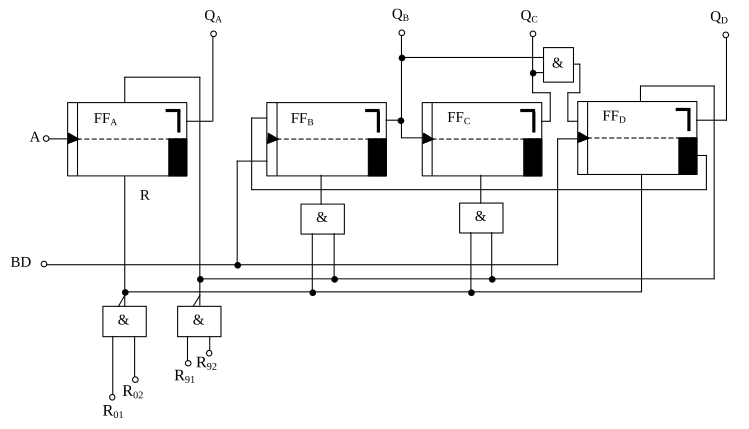
\includegraphics[width=.8\linewidth]{media/abb-51}
  \caption{Schaltbild Zähler mit Teiler}
\end{figure}

Das Prinzipschaltbild zeigt, dass auch hier 4 JK-Flipflops verwendet wurden. Hier werden zum Teil auch die Setzeingänge der Flipflops verwendet. Das bringt den Vorteil, dass Verknüpfungsschaltungen für die Rücksetzung entfallen und die Schaltung kann dadurch billiger realisiert werden.\index{Verknüpfungsschaltungen}

Als Takteingang dient hier je nach Anforderung der Eingang A oder der Eingang BD, der auch in verschiedenen Datenbüchern mit B gekennzeichnet ist.\index{Takteingang}

Mit den Eingängen R\textsubscript{01} und R\textsubscript{02} kann man eine Nullstellung „erzwingen“ indem man an beide Eingänge ein High-Signal legt. Ebenso ist es möglich mit Hilfe der beiden Eingänge R\textsubscript{91} und R\textsubscript{92} eine Neun-Stellung zu erzwingen. Mit einer entsprechenden Verknüpfungsschaltung ist es also möglich, jede Art von Zähler zwischen 0 und 9 aufzubauen indem man den Zähler beim gewünschten Stand wieder auf Null setzt. Für den Zähler von 0 bis 9 werden diese vier Eingänge auf Masse gelegt.

Den Anschluss des ICs zeigt die folgende Abbildung. Im Gegensatz zu den Transistoren werden allerdings sämtliche Pinbelegungsbilder mit den Anschlussbeinen nach unten gezeichnet. Man stellt also den IC auf die „Füße“ und betrachtet ihn von oben, nicht von unten!

\begin{figure}[htbp]
  \centering
  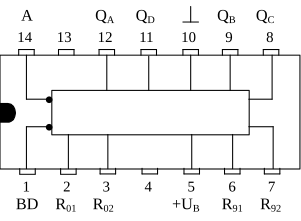
\includegraphics[width=.8\linewidth]{media/abb-52}
  \caption{IC Zähler mit Teiler}
\end{figure}

Zur Erkennung der linken oder rechten Seite eines integrierten Schaltkreises ist bei Pin 1 bzw. Pin 14 (Pin = Anschlussbeinchen) eine Kerbe oder eine punktförmige Vertiefung angebracht. Dadurch ist die Benennung des Pins sofort zu erkennen. Eingezeichnet wird dies auch auf dem Applikationsbild (Anschlussbild).

Die Anschlüsse 4 und 13 sind bei diesem Bild nicht gekennzeichnet. Das bedeutet, dass sie keinen Anschluss zur inneren Schaltung des Zählers haben. Gewöhnlich werden solche Anschlüsse mit „NC“ gekennzeichnet, was ausgeschrieben „Non Connect“ (nicht angeschlossen) heißt.

Bei Pin 14 und 1 sieht man innerhalb des ICs den Invertierungspunkt. Das bedeutet, dass bei einem L-Impuls (hier negative Flanke, da negativflankengetriggertes Flipflop) eine Umschaltung geschehen kann.

Oftmals werden auch in Datenbüchern die Benennungsbuchstaben mit einem Komplementär-Zeichen gekennzeichnet. Das wäre in diesem Fall \ensuremath{\lnot}A oder \ensuremath{\lnot}BD. Die Ausgänge Q\textsubscript{A}, Q\textsubscript{B}, Q\textsubscript{C}, Q\textsubscript{D} sind Ausgänge der Flipflops und bezeichnen die Dualstelle der dualen Zahl am Ausgang. Bei der Dualzahl 1100 hat also Q\textsubscript{D} und Q\textsubscript{C} den Wert 1, Q\textsubscript{B} und Q\textsubscript{A} haben den Wert 0.

Die Spannung wird an Pin 10 (Masse) und Pin 5 (positiver Pol der Versorgungsspannung) angeschlossen.\index{Spannung}

\section{SN 7490 als Teiler}

\subsection*{Frequenzteiler 1:2}

\begin{figure}[htbp]
  \centering
  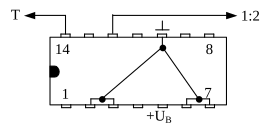
\includegraphics[width=.7\linewidth]{media/abb-53}
\end{figure}

Hierbei wird nur das Eingangsflipflop des ICs verwendet. Die vier Rückstelleingänge R\textsubscript{01}, R\textsubscript{02}, R\textsubscript{91} und R\textsubscript{92} sind mit Masse verbunden.

\subsection*{Frequenzteiler 1:3}

\begin{figure}[htbp]
  \centering
  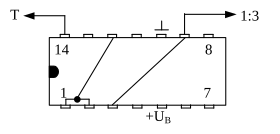
\includegraphics[width=.7\linewidth]{media/abb-54}
\end{figure}

Der Takt wird hier an den Eingang des Flipflops FF\textsubscript{A} gelegt. Der Ausgang dieses Flipflops ist mit BD verbunden. Die Ausgänge Q\textsubscript{A} und Q\textsubscript{B} sind an die Rückstelleingänge R\textsubscript{01} und R\textsubscript{02} angeschlossen.

Eine Rückstellung erfolgt dann, wenn diese beiden Ausgänge ein H-Signal aufweisen.

\subsection*{Frequenzteiler 1:5}

\begin{figure}[htbp]
  \centering
  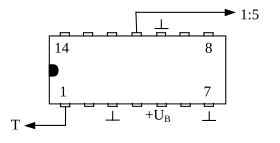
\includegraphics[width=.7\linewidth]{media/abb-55}
\end{figure}

Der Takt wird auf den Eingang BD gelegt. Somit arbeitet der Zähler nur mit der Teilerkette FF\textsubscript{B}, FF\textsubscript{C} und FF\textsubscript{D}. Durch diese Beschaltung wird ein Teilerverhältnis von 1:5 erreicht.

\subsection*{Frequenzteiler 1:9}

\begin{figure}[htbp]
  \centering
  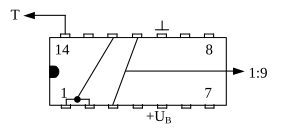
\includegraphics[width=.7\linewidth]{media/abb-56}
\end{figure}

Q\textsubscript{A} wird mit dem Flipflop-Eingang BD und mit R\textsubscript{01} verbunden. Außerdem muss Q\textsubscript{D} an R\textsubscript{02} angeschlossen werden.

Tritt nun an Q\textsubscript{A} und Q\textsubscript{D} gleichzeitig ein H-Signal auf, so wird der Zähler wieder auf 0 zurückgesetzt.

\subsection*{Frequenzteiler 1:10}

\begin{figure}[htbp]
  \centering
  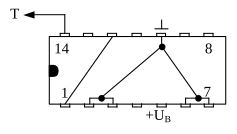
\includegraphics[width=.7\linewidth]{media/abb-57}
\end{figure}

Diese Schaltung ist nun der eigentliche Zählbetrieb des ICs. Sämtliche Rückstelleingänge sind mit Masse verbunden. Der Eingang BD der Flipflop-Kette FF\textsubscript{B}, FF\textsubscript{C} und FF\textsubscript{D} ist mit dem Ausgang Q\textsubscript{A} verbunden. An den Ausgängen Q\textsubscript{A}, Q\textsubscript{B}, Q\textsubscript{C} und Q\textsubscript{D} können nun die dualen Daten des Zählerstandes entnommen werden.

Im letzten Fall nehmen die Ausgänge also die Werte von 0000 bis 1001 (dez. 9) an. Diese Signale können nun weiter verwendet werden um z.B. einen 7-Segment-Decoder zu steuern. Dieser wiederum zeigt den Zählerstand durch ein LED Siebensegment an.\index{LED}

Zur Verdeutlichung kann man auch hier eine Logik-Tafel aufstellen. Sie sagt aus, dass eine Rückstellung nur dann erfolgen kann, wenn beide Rücksetzeingänge R\textsubscript{01} und R\textsubscript{02} (oder R\textsubscript{91} und R\textsubscript{92}) ein H-Signal erhalten.

\section{Integrierter Zähler und Teiler 7492}

Dieser IC ist ähnlich aufgebaut wie der vorher besprochene Zähler 7490. Er besteht ebenfalls aus 4 JK-Flipflops, nur sind hier andere Teilerverhältnisse zu erreichen, die im Folgenden beschrieben sind.

Das Teilerverhältnis 1:2, das nicht extra aufgeführt ist, kann man durch eine analoge Beschaltung wie beim Zähler 7490 erreichen. Auch hier wird das Eingangsflipflop für die Teilung verwendet. Wie man aus dem Prinzipschaltbild erkennt, hat dieses Bauteil keine Rücksetzung auf 9. Es ist nur eine Rückstellung auf 0 möglich. Der Eingang der Flipflopkette ist hier mit BC beschriftet. In manchen Datenbüchern wird er ebenso wie beim 7490 mit „B“ gekennzeichnet.

\begin{figure}[htbp]
  \centering
  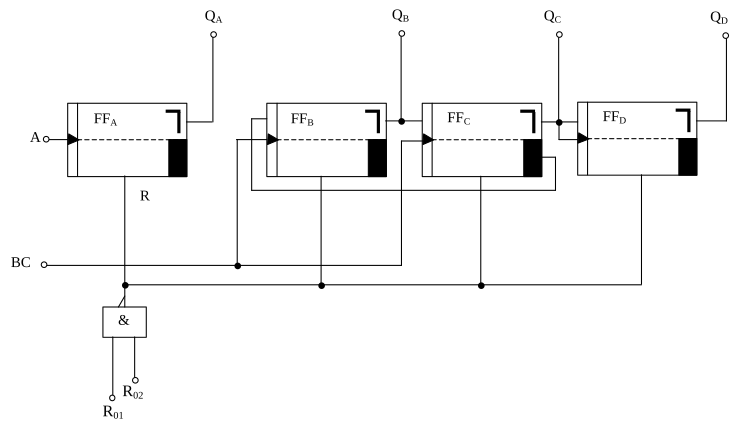
\includegraphics[width=.8\linewidth]{media/abb-58}
  \caption{Schaltbild 7492}
\end{figure}

Die Pinbelegung stimmt mit dem vorherigen Zähler in Aus- und Eingängen überein. Nur die Rückstelleingänge für 0 liegen diesmal bei Pin 6 und 7. Ohne Anschluss, also NC (Non Connect) sind die Anschlüsse 2, 3, 4 und 13. Die Stromversorgung stimmt ebenfalls mit dem Zähler 7490 überein.

\begin{figure}[htbp]
  \centering
  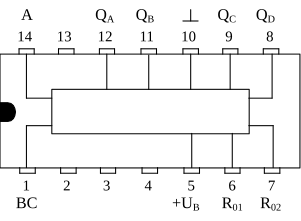
\includegraphics[width=.8\linewidth]{media/abb-59}
  \caption{IC 7492}
\end{figure}

\subsection*{Frequenzteiler 1:6}

\begin{figure}[htbp]
  \centering
  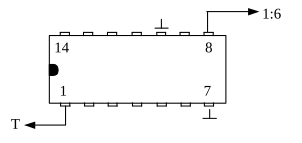
\includegraphics[width=.7\linewidth]{media/abb-60}
\end{figure}

Das Eingangsflipflop wird hier nicht verwendet. Nur die Teilerkette FF\textsubscript{B}, FF\textsubscript{C} und FF\textsubscript{D} ist angeschlossen.

\subsection*{Frequenzteiler 1:12}

\begin{figure}[htbp]
  \centering
  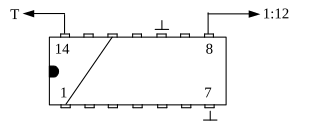
\includegraphics[width=.7\linewidth]{media/abb-61}
\end{figure}

Einer der beiden Rückstelleingänge muss auf Masse gelegt werden. Der Ausgang Q\textsubscript{A} wird mit dem Eingang BC verbunden. Somit befinden sich alle Flipflops in Betrieb.

Generell kann man an den Ausgängen der verwendeten Flipflops die H- bzw. L-Signale abgreifen. So kann man also den oberen Teiler mit Teilerverhältnis 1:6 auch als „Fünfzähler“ verwenden. Der Zähler beginnt mit der Zahl 0 und schaltet nach 5 wieder auf 0 zurück. Oder man kann mit einem Teiler 1:9 beim 7490 einen „Achterzähler“ aufbauen. Dieser beginnt ebenfalls mit der Zahl 0 zu zählen und schaltet nach der Zahl 8 auf 0 zurück.

Mit diesen Zählern kann man nun verschiedene auch für den täglichen Gebrauch sehr nützliche Schaltungen aufbauen. So z.B. eine Digitaluhr, Impulszähler, Frequenzmesser mit digitaler Anzeige, Stoppuhren und viele andere Zählschaltungen.

Doch vorerst haben wir nur das duale Signal. Dieses muss durch eine geeignete Decoderschaltung in ein sichtbares, sofort erkennbares Signal umgeformt werden. Bei unseren Zählerschaltungen empfiehlt sich die Umformung in einen Code, der durch eine 7-Segmentanzeige angezeigt werden kann. Ein solcher Decoder kann durch geeignete Verknüpfungsschaltungen aufgebaut werden. Da diese Schaltung aber sehr umfangreich würde, empfiehlt es sich auch hier auf einen schon fertigen Decoder zurückzugreifen, wie er im nächsten Kapitel beschrieben wird.\index{Verknüpfungsschaltungen}

\section{BCD-to-7-Segment Decoder}

Die Abkürzung BCD steht für „binary coded decimal“ und meint einfach die binäre Darstellung einer Dezimalzahl. Ein BCD-to-7-Segment Decoder wandelt nun ein solches Signal in entsprechende Steuersignale für eine 7-Segmentanzeige um. Das bedeutet, dass ein duales Signal an die Eingänge dieser Schaltung gelegt wird und dieses Signal in einen Code für die 7-Segmentanzeige umgewandelt wird. Aber was ist jetzt eigentlich eine 7-Segmentanzeige?

Eine solche Anzeige besteht aus 7 LEDs (Licht emittierende Dioden). Eine Leuchtdiode sendet Licht aus, wenn sie in Durchlassrichtung geschaltet ist. Das Material ist meist Galliumarsenid. Das Leuchten entsteht in dem Grenzgebiet zwischen der n- und der p-Zone des Halbleiterelements, durch die Energie der bewegten Ladungsträger. Der Durchlassstrom, der zum Leuchten durch die Diode fließen muss, liegt bei etwa 1 mA. Dies ist eine ideale Voraussetzung für die am Ausgang nicht stark belastbaren Gatterschaltungen. Somit hat eine Leuchtdiode gegenüber einer normalen Glühlampe den Vorteil, dass zum Aussenden von Licht ein weitaus geringerer Strom benötigt wird, und somit eine umfangreiche Schaltung zur Stromverstärkung entfallen kann.

Unterschiede zwischen verschiedenen Leuchtdioden gibt es nicht nur in der Leuchtfarbe (rot, gelb, grün, blau, weiß), sondern auch in der Bauteilgröße: Von Subminiatur bis Normal-Grösse sind sie im Handel erhältlich, je nach Geschmack und Anforderung.

Die 7-Segmentanzeige wird überall dort verwendet, wo Zahlen angezeigt werden sollen, z.B. in Taschenrechnern und digitalen Uhren. Die Anordnung der 7 LEDs ist so gewählt, dass jede Ziffer zwischen 0 und 9 und einige Sondersymbole dargestellt werden können. Um eine einheitliche Benennung der Segmente zu erreichen, werden die einzelnen Leuchtdioden mit den kleinen Buchstaben a, b, c, d, e, f und g benannt.

\begin{figure}[htbp]
  \centering
  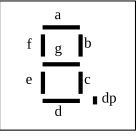
\includegraphics[width=.8\linewidth]{media/abb-62}
  \caption{7-Segment Anzeige}
\end{figure}

Um die Ziffer 0 mit einer solchen Anzeige aufleuchten zu lassen, müssen die Segmente a, b, c, d, e und f zum Leuchten gebracht werden. Und genau diese Aufgabe übernimmt der Decoder. Das duale Signal, das z.B. von einem Zähler kommen kann, ist im Fall der Ziffer 0 ein 0-Wert an allen Eingängen, also 0000. Oder anders ausgedrückt: Die Ausgänge Q\textsubscript{A}, Q\textsubscript{B}, Q\textsubscript{C} und Q\textsubscript{D} eines Zählers, die gleichzeitig die Eingänge des Decoders sind, haben bei der dezimal angezeigten Zahl 0 alle den Wert 0. Intern wird dieses angelegte Signal weiterverarbeitet, um als dezimale Ziffer auf der 7-Segmentanzeige angezeigt werden zu können.

Ein solcher BCD-to-7-Segment Decoder ist z.B. der IC „SN 7447“. Die Pinbelegung ist in Abb. 54 zu sehen. Die Versorgungsspannung liegt an Pin 8 und 16, die Ausgänge a, b, c, d, e, f und g an den Pins 9 bis 15. Diese Ausgänge sind innerhalb der Schaltung invertiert, d.h. bei einem 1-Signal liegt am Ausgang der Wert 0 (was dem Minuspol der Spannungsquelle entspricht). Da 7-Segmentanzeigen mit gemeinsamer Anode und gemeinsamer Kathode angeboten werden, muss bei einer Invertierung der Ausgänge immer eine Anzeige mit gemeinsamer Anode genommen werden. Die Anode wird an den Pluspol der Versorgungsspannung angeschlossen. Der Minuspol (Masseanschluss) entspricht dem Wert 0 und wird vom Decoder am Ausgang geliefert.\index{Spannungsquelle}\index{Masseanschluss}

\begin{figure}[htbp]
  \centering
  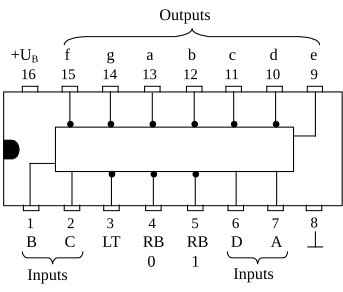
\includegraphics[width=.8\linewidth]{media/abb-63}
  \caption{IC BCD nach 7-Segment Decoder}
\end{figure}

Beim Anschluss der 7-Segmentanzeige wird zuerst der gemeinsame Anoden-Pin an den Pluspol der Versorgungsspannung angeschlossen. Der Anschluss „dp“, der für den Dezimalpunkt vorgesehen ist, kann offen gelassen werden. Um ihn zu steuern, ist eine weitere Verknüpfung notwendig. Verwendet wird er z.B. beim Taschenrechner, um die Kommastelle zu markieren. Für einen Zählerbausatz ist dies aber nicht unbedingt notwendig.

Der Anschluss „LT“ ist ein Lampentest-Eingang, der durch einen Masseanschluss aktiviert werden kann. Masseanschluss deshalb, weil auch hier intern eine Invertierung vorgenommen wird. Ist dieser Pin an den Massepool angeschlossen, so leuchten sämtliche Segmente für diese Zeit auf. Somit ist ein Test der einzelnen Leuchtdioden möglich. Weiterhin ist eine Helligkeitssteuerung und eine Unterdrückung von führenden Nullen möglich.\index{Masseanschluss}

Die Anzeige der einzelnen Segmente zeigt Abb. 55. Unter den schematischen Segmentbildern ist der Zählerstand beim Decodereingang aufgezählt. Wie man sieht, erscheinen ab der Zahl 10 Sondersymbole. Dies kommt daher, dass mit einem Segment nur Zahlen von 0 bis 9 möglich sind, der Decoder aber durch die vier Eingänge bis zur dualen Zahl 1111 (dezimal 15) zu steuern ist.

\begin{figure}[htbp]
  \centering
  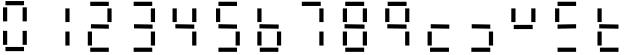
\includegraphics[width=.8\linewidth]{media/abb-64}
  \caption{7-Segment Anzeige}
\end{figure}

\section{Dezimalzähler mit Anzeige (7-Segment)}

Dies ist eine Kombination des Dezimalzählers SN 7490 und des BCD-to-7-Segment Decoders SN 7447. Der Decoder gibt das empfangene Signal des Zählers umgeformt an die 7-Segment-Anzeige mit gemeinsamer Anode weiter. Das Taktsignal (z.B. von einem Taktgeber) wird an den rechten Zähler gelegt. Durch seine Beschaltung zählt er von 0 bis 9, kehrt danach auf 0 zurück und beginnt von Neuem mit dem Zählvorgang. Das erreicht man, wie schon beschrieben, indem man die Rücksetzeingänge R\textsubscript{01}, R\textsubscript{02}, R\textsubscript{91} und R\textsubscript{92} (hier mit Reset bezeichnet) auf Masse legt. Außerdem muss der Ausgang Q\textsubscript{A} mit dem Eingang BD verbunden werden. Der Zähler gibt nun sein Signal an den Decoder weiter. Dabei werden die Ausgänge des Zählers mit den dazugehörigen Eingängen des Decoders verbunden, d.h. der Ausgang Q\textsubscript{A} mit dem Eingang A usw.\index{Taktgeber}

Der Decoder formt das Signal des Dezimalzählers in einen Code um, der durch die 7-Segment-Anzeige als Zahl sichtbar wird.

Die Steuerung des zweiten Zählers erfolgt bei der Rücksetzung des ersten Zählers auf 0. Der Ausgang Q\textsubscript{D} des ersten Zählers, der ab der Zahl 8 (entspr. 1000) den Wert 1 hat, erzeugt bei der Rückstellung eine negative Flanke, die für eine Taktung des zweiten Zählers ausgenutzt wird. Das Spannungsdiagramm dieses Ausgangs ist unten abgebildet.

\begin{figure}[htbp]
  \centering
  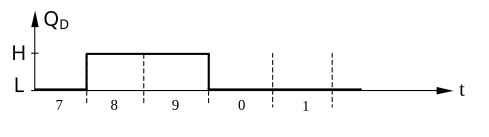
\includegraphics[width=.8\linewidth]{media/abb-65}
  \caption{Spannungsdiagramm}
\end{figure}

Mit diesem Schaltungsschema können nun beliebig viele Zähler aneinander gereiht werden.

Bei dem vorliegenden Zähler ist ein Zählerstand von 00 bis 99 möglich. Nicht zu vergessen ist, dass die gemeinsame Anode der 7-Segment-Anzeige an den Pluspol der Versorgungsspannung angeschlossen werden muss. Ebenso ist es noch nötig die Stromversorgung, die hier nicht eingezeichnet wurde, an die Zähler und die Decoder anzuschließen.

Getaktet wird die ganze Schaltung mit einem der besprochenen Taktgeber, also entweder mit Einzelimpulsen oder Folgeimpulsen.\index{Taktgeber}

\begin{figure}[htbp]
  \centering
  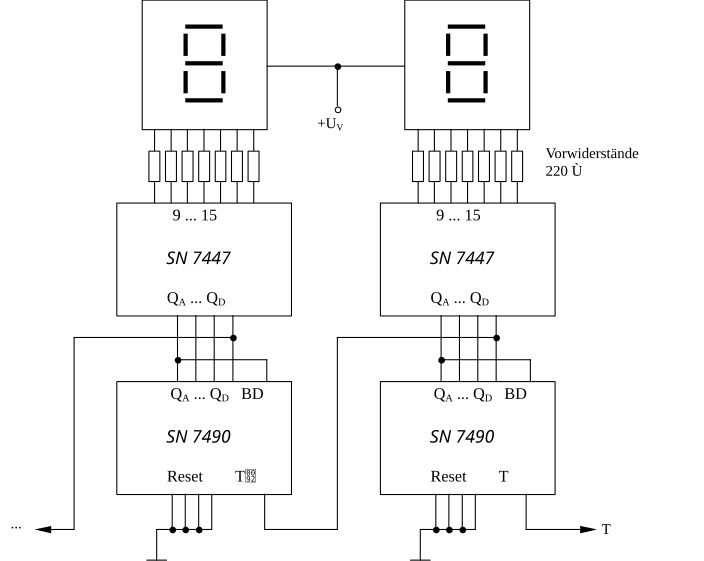
\includegraphics[width=.8\linewidth]{media/abb-66}
  \caption{Schaltbild Dezimalzähler mit 7-Segmentanzeige}
\end{figure}

\section{BCD-to-Decimal Decoder}

Diese Schaltung ist eine weitere Decoderschaltung. Sie setzt nicht wie beim vorherigen Decoder das duale Signal (BCD-Signal) in ein Signal für eine 7-Segment-Anzeige um, sondern liefert ein dezimales Signal. Das heißt konkret, dass bei einem gewissen Zählerstand des Eingangs ein Signal an einem bestimmten Ausgang erscheint. Wird z.B. an den Eingang des Decoders das duale Signal 0000 gelegt, das der dezimalen Zahl 0 entspricht, so erhält der Ausgang mit der Nummer 0 das Signal. Oder, um ein weiteres Beispiel zu nennen, wenn am Eingang das duale Signal 0110 angelegt wird (entspr. dezimal 6) so liegt am Ausgang 6 das ausgehende Signal.

\begin{figure}[htbp]
  \centering
  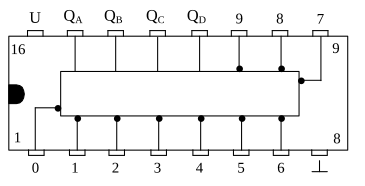
\includegraphics[width=.8\linewidth]{media/abb-67}
  \caption{IC BCD nach Dezimal Decoder}
\end{figure}

Abb. 57 zeigt einen solchen BCD-to-Decimal Decoder, es ist der IC „SN 7445“. Wie man sieht, hat er genau 10 Ausgänge, beschriftet mit „0“ bis „9“. An ihnen kann das invertierte Signal, also ein L-Wert, abgegriffen werden. An die Eingänge Q\textsubscript{A}, Q\textsubscript{B}, Q\textsubscript{C} und Q\textsubscript{D} wird das duale Signal, das z.B. von einem Dezimalzähler kommen kann, angelegt.

Da der Decoder nur Ausgänge von 0 bis 9 hat, können nur duale Zahlen bis einschliesslich 1001 decodiert werden. Diese Zahl entspricht genau der dezimalen Zahl 9. Die angelegten Werte über dieser Grenze, also Zahlen von 10 bis 15 bewirken keine Signalübermittlung an den Ausgängen. An ihnen erscheint dann generell der Wert 1, da ja die Ausgänge invertiert sind.

Dieser Schaltkreis kann z.B. eine LED-Kette steuern. Dazu wird an die Eingänge Q\textsubscript{A}, Q\textsubscript{B}, Q\textsubscript{C} und Q\textsubscript{D} das Signal eines Dezimalzählers angeschlossen. Man kann nun genau ablesen, welchen Zählerstand der Dezimalzähler gerade hat. Wechseln die einzelnen Werte am Eingang des Decoders in schnelleren Schritten, d.h. wird an den Zähler eine höhere Taktfrequenz angelegt, so erhält man ein Lauflicht. Die dunkle Leuchtdiode wechselt ihre Position bei jeder Zählerstandsänderung.\index{LED}\index{Taktfrequenz}


\chapter{Schieberegister}

\section{Einführung}

Auch bei den sogenannten Schieberegistern finden JK-Flipflops Anwendung. Maßgeblich beteiligt sind dabei nur die Eingänge J und K, der Takteingang T und, wenn erforderlich, der Rücksetzeingang R.\index{Takteingang}\index{Rücksetzeingang}

Ein Schieberegister ist so aufgebaut, dass der Taktimpuls an alle Takteingänge gleichzeitig gelegt wird. Es findet also keine Taktteilung statt, sondern alle Flipflops haben den selben Takt. Weiterhin wird jeweils der Q-Ausgang des vorhergehenden Flipflops mit dem J-Eingang des nachfolgenden Flipflops verbunden und der \ensuremath{\lnot}Q-Ausgang mit dem K-Eingang.\index{Taktimpuls}

Der Dateneingang D dieser Kette wird an den Eingang des ersten Flipflops gelegt und invertiert an den K-Eingang.\index{Dateneingang}

\begin{figure}[htbp]
  \centering
  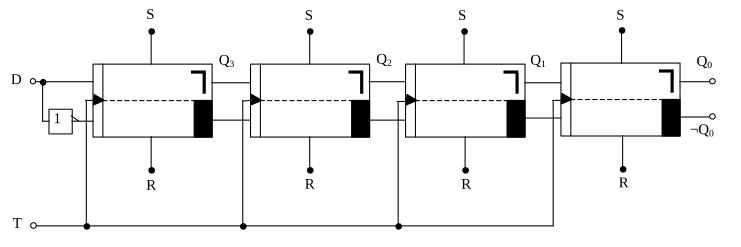
\includegraphics[width=.8\linewidth]{media/abb-68}
  \caption{Schaltbild Schieberegister}
\end{figure}

Wird bei dieser Schaltung an den Takteingang T ein Impuls gelegt, so wird die gespeicherte Information des Flipflops 3 an die Eingänge des Flipflops 2 weiter „geschoben“. Daher auch der Begriff „Schieberegister“. Die an D angelegten Daten werden also mit jedem Taktimpuls um eine Flipflopstelle weiter nach rechts geschoben. In diesem Beispiel können im Höchstfall 4 Werte in den Flipflops gespeichert werden. Es handelt sich dabei also um ein „4-Bit-Schieberegister“. Ein Bit stellt eine Informationseinheit dar und hat entweder den Wert 0 oder den Wert 1.\index{Takteingang}\index{Taktimpuls}

Spielen wir nun einmal einen solchen Ablauf durch. An den Dateneingang D wird der Wert 1 gelegt. Wird nun ein Taktimpuls wirksam, so erhält das Flipflop 3 am Ausgang Q\textsubscript{3} den Wert 1. Daraufhin wird an D der Wert 0 angelegt. Mit dem nächsten Taktimpuls an T wird der Wert 1 von FF\textsubscript{3} an FF\textsubscript{2} weitergeschoben; es tritt also an FF\textsubscript{2} der Wert 1 am Ausgang auf. Außerdem wird beim selben Taktimpuls der Datenwert 0 vom Eingang D auf das FF\textsubscript{3} übernommen, womit am Ausgang Q\textsubscript{3} der Wert 0 auftritt. Wird nun an den Eingang D der Wert 1 gelegt und tritt ein erneuter Taktimpuls auf, so erhält der Ausgang Q\textsubscript{1} den Wert 1, Q\textsubscript{2} erhält den Wert 0 und Q\textsubscript{3} den Wert des Dateneingangs vor dem Impuls, also 1. Wird daraufhin an D der Wert 0 gelegt und wird ein neuer Taktimpuls wirksam, so erscheint am Ausgang Q\textsubscript{3} der Wert 0, an Q\textsubscript{2} der Wert 1, an Q\textsubscript{1} der Wert 0 und an Q\textsubscript{0} der Wert 1.\index{Dateneingang}\index{Taktimpuls}

Der angelegte Wert von D wird also immer pro Taktimpuls um eine Stelle weiter geschoben.\index{Taktimpuls}

Die folgende Tabelle zeigt den Sachverhalt der Verschiebung anschaulich. Dabei sind die Informationen, d.h. die Werte 1 oder 0, die an D gelegt werden durch die Variablen a\textsubscript{3}, a\textsubscript{2}, a\textsubscript{1} und a\textsubscript{0} ersetzt. Wichtig dabei ist, dass man zuerst die Daten für a\textsubscript{0} eingeben muss, dann die für a\textsubscript{1} usw., damit am Ende die Datenreihe a\textsubscript{3}a\textsubscript{2}a\textsubscript{1}a\textsubscript{0} erreicht wird. Ein X in der Tabelle bedeutet, dass der Wert an dieser Stelle beliebig ist.

\begin{table}[htbp]
  \centering
  \begin{tabular}{cccccc}
    \toprule
    t & D & Q\textsubscript{3} & Q\textsubscript{2} & Q\textsubscript{1} & Q\textsubscript{0} \\
    \midrule
    0 & D=a\textsubscript{0} & X & X & X & X \\
    1 & D=a\textsubscript{1} & a\textsubscript{0} & X & X & X \\
    2 & D=a\textsubscript{2} & a\textsubscript{1} & a\textsubscript{0} & X & X \\
    3 & D=a\textsubscript{3} & a\textsubscript{2} & a\textsubscript{1} & a\textsubscript{0} & X \\
    4 & X & a\textsubscript{3} & a\textsubscript{2} & a\textsubscript{1} & a\textsubscript{0} \\
    \bottomrule
  \end{tabular}
\end{table}

Eine weitere Möglichkeit der Eingabe der 4 Daten ist durch die Möglichkeit des Setzens gegeben. Die Daten können nämlich auch durch die Setz- bzw. Rücksetzeingänge eingegeben werden, soweit diese vorhanden sind. Dabei ist ja, wie bekannt, kein Takt nötig.

Falls die Rücksetzeingänge bei einer „Taktsetzung“ (also einer Registrierung der Daten über die J- und K-Eingänge) miteinander verbunden sind, kann damit das ganze Register gelöscht werden. Dies ist von großem Vorteil bei einem Ringschieberegister, das folgend abgebildet ist.\index{Ringschieberegister}

\begin{figure}[htbp]
  \centering
  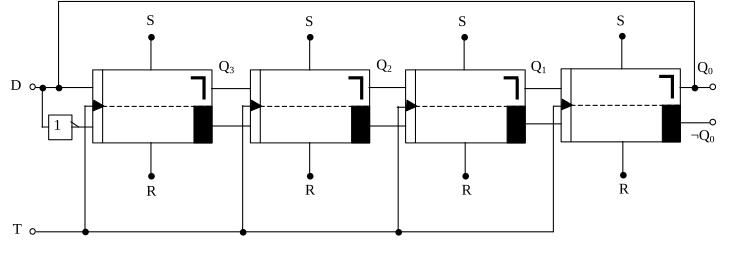
\includegraphics[width=.8\linewidth]{media/abb-69}
  \caption{Schaltbild Schieberegister}
\end{figure}

Bei diesem Ringschieberegister ist der Ausgang Q\textsubscript{0} mit dem Dateneingang D verbunden. Die Daten werden also in einem Ring weitergeschoben. Dadurch bleiben die einmal gespeicherten Werte die ganze Zeit über gespeichert. Bei einem normalen Schieberegister müsste man ständig bei D neue Daten eingeben, während beim Ringschieberegister die einmal gespeicherten Bits erhalten bleiben und nur ihren Platz wechseln. Die Registrierung der Daten bei einem solchen Ringschieberegister erfolgt zweckmäßigerweise über die Setz- bzw. Rücksetzeingänge. Es ist aber auch eine Registrierung über die J- und K-Eingänge möglich. Nur muss in diesem Fall für die Zeit der Dateneingabe die Verbindung zwischen Q\textsubscript{0} und R unterbrochen werden, da Ausgänge generell nicht zusammengeschaltet werden dürfen. Diese Trennung kann z.B. über eine Verknüpfungsschaltung geschehen.\index{Ringschieberegister}\index{Dateneingang}\index{Ringschieberegister}

Um eine Vereinfachung der Schaltung zu erreichen, hat man für das Schieberegister ein Schaltsymbol entworfen, ebenso für das Ringschieberegister.\index{Ringschieberegister}

\begin{figure}[htbp]
  \centering
  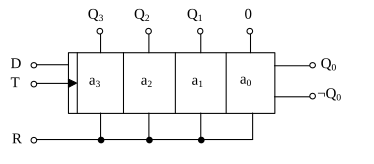
\includegraphics[width=.8\linewidth]{media/abb-70}
  \caption{Schaltsymbol Schieberegister}
\end{figure}

An den Takteingang T wird der Takt angelegt. Die Daten werden über den Dateneingang D in die Register a\textsubscript{3}, a\textsubscript{2}, a\textsubscript{1} und a\textsubscript{0} geschoben und können an den Ausgängen Q\textsubscript{3}, Q\textsubscript{2}, Q\textsubscript{1} und Q\textsubscript{0} bzw. \ensuremath{\lnot}Q\textsubscript{0} abgegriffen werden. Mit dem Rücksetzeingang R kann das gesamte Register gelöscht werden.\index{Takteingang}\index{Dateneingang}\index{Rücksetzeingang}

\begin{figure}[htbp]
  \centering
  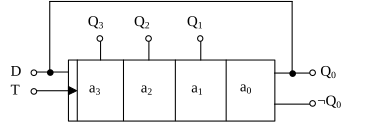
\includegraphics[width=.8\linewidth]{media/abb-71}
  \caption{Schaltsymbol Schieberegister}
\end{figure}


\chapter{Volladdierer}

\section{Einführung}

Ein Volladdierer ist eine Schaltung, die zwei Dualzahlen zusammenzählt. Dabei beginnt er bei der letzten Stelle, genau so, wie eine Addition „von Hand“ ausgeführt wird. Hier ein kleines Beispiel:\index{Volladdierer}\index{Addition}

Die Dualzahlen a\textsubscript{3}a\textsubscript{2}a\textsubscript{1}a\textsubscript{0} und b\textsubscript{3}b\textsubscript{2}b\textsubscript{1}b\textsubscript{0} sollen addiert werden.

\begin{table}[htbp]
  \centering
  \begin{tabular}{ccccc}
    \toprule
     & a\textsubscript{3} & a\textsubscript{2} & a\textsubscript{1} & a\textsubscript{0} \\
    \midrule
    + & b\textsubscript{3} & b\textsubscript{2} & b\textsubscript{1} & b\textsubscript{0} \\
     & Ü\textsubscript{3} & Ü\textsubscript{2} & Ü\textsubscript{1} &  \\
    Ü\textsubscript{4} & S\textsubscript{3} & S\textsubscript{2} & S\textsubscript{1} & S\textsubscript{0} \\
    \bottomrule
  \end{tabular}
\end{table}

Die Dualzahlen werden untereinander geschrieben. Danach wird die Summe aus a\textsubscript{0} + b\textsubscript{0} gebildet und der Übertrag Ü\textsubscript{1} unter a\textsubscript{1} und b\textsubscript{1} geschrieben. So läuft die Addition weiter bis zum Übertrag Ü\textsubscript{4}, der vor die Summen S\textsubscript{3} S\textsubscript{2} S\textsubscript{1} S\textsubscript{0} gesetzt wird.\index{Addition}

Dabei kann der Volladdierer (VA) nur zwei einstellige Dualzahlen addieren, wodurch ein kleiner Kunstgriff nötig wird um größere Dualzahlen zu addieren. Doch dazu später mehr.\index{Volladdierer}

Zuerst stellt sich die Frage: Wie werden Dualzahlen eigentlich addiert? Dabei gelten natürlich genau wie bei der Addition im Dezimalsystem auch bestimmte Regeln. Diese sind in der Logik-Tafel abgebildet. Dabei stellt A eine zu addierende Variable dar, B die andere. Diese beiden Werte A und B werden also zu der Summe S und dem Übertrag Ü zusammengefasst.\index{Addition}\index{Dezimalsystem}

\begin{table}[htbp]
  \centering
  \begin{tabular}{cccc}
    \toprule
    A & B & S & Ü \\
    \midrule
    0 & 0 & 0 & 0 \\
    0 & 1 & 1 & 0 \\
    1 & 0 & 1 & 0 \\
    1 & 1 & 0 & 1 \\
    \bottomrule
  \end{tabular}
\end{table}

Ein Volladdierer besteht eigentlich aus zwei Halbaddierern, die zwei einstellige Dualzahlen addieren können, jedoch ohne Übertrag. Durch die Zusammenschaltung dieser beiden Halbaddierer ist es möglich, eine Summe samt Übertrag zu bilden. Da die Volladdierer aber als fertige ICs angeboten werden, empfiehlt es sich, diese zu verwenden.\index{Volladdierer}\index{Halbaddierer}

Doch nun zu dem vorher angesprochenen Problem. Wie sieht eine Volladdierer-Schaltung aus, mit der man zwei vierstellige Dualzahlen summieren kann?\index{Volladdierer}

Bei diesem Problem hilft uns wiederum das Schieberegister. Wenn man die Register mit den schon gespeicherten Daten an einen VA in der angegebenen Weise anschliesst, so stehen pro Taktimpuls immer nur zwei Werte der beiden Dualzahlen zur Addition zur Verfügung. Es beginnt mit den beiden Werten a\textsubscript{0} und b\textsubscript{0}. Diese werden nun in den VA eingegeben, der sie addiert. Am Ausgang S steht dann die Summe dieser beiden Zahlen und am Ausgang Ü der Übertrag. Bei einem erneuten Taktimpuls gelangen nun die beiden Dualwerte a\textsubscript{1} und b\textsubscript{1}, die ja nach dem letzten Taktimpuls den Platz von a\textsubscript{0} und b\textsubscript{0} eingenommen haben, an den VA.\index{Taktimpuls}\index{Addition}

Das JK-Flipflop unterhalb der Schieberegister, das vor diesem Taktimpuls den Wert Ü\textsubscript{1} am Eingang hatte, hat nun den Wert Ü\textsubscript{1} am Ausgang Q. Dieser Ausgang Q ist nun mit einem weiteren Eingang C des VA verbunden. Es liegen also an den Eingängen des Volladdierers die Werte a\textsubscript{1} (an A), b\textsubscript{1} (an B) und Ü\textsubscript{1} an C. Diese werden wiederum addiert und erscheinen als Summe S und als Übertrag Ü an dessen Ausgängen.\index{JK-Flipflop}\index{Taktimpuls}

Zuvor wurde jedoch der Ausgang S des VA mit dem J-Eingang des Serienaddierers verbunden. Nachdem nun die Summe a\textsubscript{0} + b\textsubscript{0} gebildet wurde und ein erneuter Taktimpuls die Werte a\textsubscript{3}, a\textsubscript{2} und a\textsubscript{1} um eine Stelle weiter nach rechts geschoben hat (ebenso die Werte b\textsubscript{3}, b\textsubscript{2} und b\textsubscript{1}), sind in den Schieberegistern folgende Werte gespeichert.\index{Taktimpuls}

\begin{quote}
  Register A: X,  a\textsubscript{3}, a\textsubscript{2}, a\textsubscript{1}
\end{quote}


\begin{quote}
  Register B: S\textsubscript{0}, b\textsubscript{3}, b\textsubscript{2}, b\textsubscript{1}
\end{quote}


In dem JK-Flipflop befindet sich der Übertrag Ü\textsubscript{1}.\index{JK-Flipflop}

Nun tritt die erneute Addition der Variablen an A, B und C des VA auf. Es wird also die Summe a\textsubscript{1} + b\textsubscript{1} + Ü\textsubscript{1} gebildet. Dabei wird die Summe S\textsubscript{1} gebildet, die wiederum am J-Eingang des unteren Schieberegisters anliegt und bei einem erneuten Taktimpuls als Information aufgenommen wird. Der Übertrag Ü\textsubscript{2}, der bei der Addition entsteht und an den J-Eingang des Flipflops gelegt wird, wird auch von diesem beim nächsten Impuls aufgenommen und erscheint dann am Ausgang Q um von dort bei einer erneuten Addition übernommen zu werden.\index{Addition}\index{Taktimpuls}

Es befinden sich also jetzt folgende Werte in den Registern:

\begin{quote}
  Register A: X,   X, a\textsubscript{3}, a\textsubscript{2}
\end{quote}


\begin{quote}
  Register B: S\textsubscript{1}, S\textsubscript{0}, b\textsubscript{3}, b\textsubscript{2}
\end{quote}


In dem JK-Flipflop befindet sich der Übertrag Ü\textsubscript{2}.\index{JK-Flipflop}

Bei einem erneuten Taktimpuls wird die Summe der Werte a\textsubscript{2}, b\textsubscript{2} und Ü\textsubscript{2} gebildet. Es erscheint dann am Ausgang S des VA die gebildete Summe S\textsubscript{2} und der Übertrag Ü\textsubscript{3}.\index{Taktimpuls}

Diese Art der Addition wird so weit fortgesetzt bis sämtliche Variablen addiert sind. Nachdem die letzte Summierung geschehen ist und die letzte Summe in dem unteren Schieberegister abgespeichert wurde, sind die Werte wie folgt in den Registern:\index{Addition}

Register A: X,   X,  X,  X

Register B: S\textsubscript{3}, S\textsubscript{2}, S\textsubscript{1}, S\textsubscript{0}

In dem JK-Flipflop befindet sich der Übertrag Ü\textsubscript{4}.\index{JK-Flipflop}

Der Übertrag Ü\textsubscript{4} kann nun aus dem JK-Flipflop entnommen werden und vor die Summe S\textsubscript{3}, S\textsubscript{2}, S\textsubscript{1}, S\textsubscript{0} gesetzt werden. Der Sachverhalt der Verschiebung innerhalb des Registers und die Addition der einzelnen Variablen zu einer Summe S und dem Übertrag Ü ist in der folgenden Tabelle noch einmal zusammengefasst.\index{JK-Flipflop}\index{Addition}

Schieberegister A:

\begin{table}[htbp]
  \centering
  \begin{tabular}{ccccc}
    \toprule
    t & Stelle 3 & Stelle 2 & Stelle 1 & Stelle 0 \\
    \midrule
    0 & a\textsubscript{3} & a\textsubscript{2} & a\textsubscript{1} & a\textsubscript{0} \\
    1 & X & a\textsubscript{3} & a\textsubscript{2} & a\textsubscript{1} \\
    2 & X & X & a\textsubscript{3} & a\textsubscript{2} \\
    3 & X & X & X & a\textsubscript{3} \\
    4 & X & X & X & X \\
    \bottomrule
  \end{tabular}
\end{table}

Schieberegister B:

\begin{table}[htbp]
  \centering
  \begin{tabular}{ccccc}
    \toprule
    t & Stelle 3 & Stelle 2 & Stelle 1 & Stelle 0 \\
    \midrule
    0 & b\textsubscript{3} & b\textsubscript{2} & b\textsubscript{1} & b\textsubscript{0} \\
    1 & S\textsubscript{0} & b\textsubscript{3} & b\textsubscript{2} & b\textsubscript{1} \\
    2 & S\textsubscript{1} & S\textsubscript{0} & b\textsubscript{3} & b\textsubscript{2} \\
    3 & S\textsubscript{2} & S\textsubscript{1} & S\textsubscript{0} & b\textsubscript{3} \\
    4 & S\textsubscript{3} & S\textsubscript{2} & S\textsubscript{1} & S\textsubscript{0} \\
    \bottomrule
  \end{tabular}
\end{table}

JK-Flipflop:\index{JK-Flipflop}

\begin{table}[htbp]
  \centering
  \begin{tabular}{cc}
    \toprule
    t & Q \\
    \midrule
    0 & X \\
    1 & Ü\textsubscript{1} \\
    2 & Ü\textsubscript{2} \\
    3 & Ü\textsubscript{3} \\
    4 & Ü\textsubscript{4} \\
    \bottomrule
  \end{tabular}
\end{table}

\begin{figure}[htbp]
  \centering
  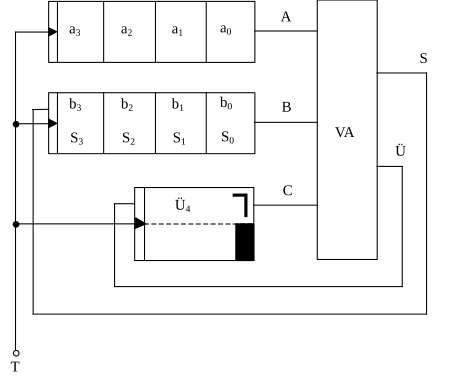
\includegraphics[width=.8\linewidth]{media/abb-72}
  \caption{Schaltbild Serienaddierer}
\end{figure}

Das obere Schieberegister A, das untere B, das JK-Flipflop und der Volladdierer bilden zusammen eine Einheit. Da diese Schaltung mehrere Variablen, also eine „Serie von Bits“, addieren kann, nennt man diese Schaltung auch einen Serienaddierer.\index{JK-Flipflop}\index{Volladdierer}

Der Takt T, der an den beiden Schieberegistern und dem Flipflop liegt muss an den Eingang T angelegt werden. Weiterhin müssen die dualen Zahlen a\textsubscript{3}a\textsubscript{2}a\textsubscript{1}a\textsubscript{0} und b\textsubscript{3}b\textsubscript{2}b\textsubscript{1}b\textsubscript{0} über die Setz- und Rücksetzeingänge in die Register geladen werden. Diese Eingänge sind hier der Übersicht wegen nicht eingezeichnet.

Wenn die Schaltung aufgebaut und in Betrieb genommen wird, empfiehlt es sich zuerst Einzelimpulse an den Takteingang T zu legen. So kann die Schaltung Schritt für Schritt beobachtet  und kontrolliert werden. Danach ist ein Betrieb mit höherer Taktfrequenz möglich.\index{Takteingang}\index{Taktfrequenz}



\backmatter
% Kapitel 12 des Manuskripts war der Anhang, und der bestand nur aus dem
% Abbildungs- und dem Stichwortverzeichnis. Beide setzt LaTeX selbst, mit
% eigenen Seitenzahlen - der alte Text dazu ist deshalb nicht eingebunden.
\listoffigures
\printindex

\end{document}
